\documentclass[acmtog]{acmart}
\setcopyright{none}
\citestyle{acmauthoryear}
\settopmatter{printacmref=false,printccs=false,printfolios=true}
\renewcommand\footnotetextcopyrightpermission[1]{}
\usepackage[T1]{fontenc}
\usepackage[utf8]{inputenc}
\usepackage{textcomp}
\usepackage{amsmath}
\usepackage{booktabs,array,tabularx,multirow}
\usepackage{graphicx}
\usepackage{tikz}
\usepackage{xcolor}
\usepackage{microtype}
\usepackage{siunitx}
\usepackage{enumitem}
\usepackage{url}
\usepackage{bookmark}
\setlength{\emergencystretch}{3em}
\setlength{\textfloatsep}{9pt plus 2pt minus 2pt}
\setlength{\floatsep}{7pt plus 2pt minus 2pt}
\providecommand{\tightlist}{\setlength{\itemsep}{0pt}\setlength{\parskip}{0pt}}
\sisetup{round-mode=places,round-precision=3,detect-weight=true}
\hypersetup{hidelinks,pdftitle={Reality Probe: Information-Limited Physical Verification of Captured Worlds},pdfauthor={Swayam Singal}}
\title{Reality Probe: Information-Limited Physical Verification of Captured Worlds}
\author{Swayam Singal}
\email{swayam.singal@gmail.com}
\keywords{captured worlds, inverse physics, physical verification, counterfactual simulation, material point method, uncertainty, experiment design, Gaussian splatting}
\begin{document}
\begin{abstract}
A captured scene can now carry enough physical state to be simulated, edited, and replayed after capture. That makes physical editing possible, but it also creates a verification problem: a rewrite can reduce ordinary held-out error while making an untouched physical behavior worse. We study this failure mode and introduce Reality Probe, a rewrite-level verification contract that separates proposal generation from a reserved physical test and returns SUPPORT, VETO, or UNRESOLVED according to a fixed evidence rule. The experiments deliberately include both successful and failed verification channels. Dark-Field Counterfactual Spectroscopy (DCS), a signed intervention contrast used inside Reality Probe, passes a constructed control but resolves none of the proposals in several frozen synthetic regimes. A separately frozen known-force compliance channel increases median standardized evidence magnitude by 11.46$\times$, yet all 36 fresh synthetic proposals remain below the decision boundary. On a repository-locked IRIS pendulum final set, a finite-amplitude period probe makes 90/110 controlled decisions correctly, compared with 40/110 for a matched small-angle diagnostic baseline; the 110 cases are nested within 10 physical videos, and all 10 placebo cases are correctly left UNRESOLVED. The result does not transfer automatically to another equation family. A frozen IRIS free-fall validation run passes low-level quality checks on 5/5 videos but reaches 111.7\% median acceleration relative error, so the lane is closed and its final split remains unopened. These results support a conditional systems claim: verification is useful when the reserved physical channel contains information that separates the candidate rewrite from the baseline, and abstention is the correct outcome when it does not.
\end{abstract}

\maketitle
\pagestyle{plain}
\thispagestyle{plain}

\section{Introduction}\label{introduction}

Consider a captured object whose simulated material parameters have been fitted from video. An optimizer proposes a new parameter set because it lowers error on ordinary held-out frames. That improvement answers a fitting question: the rewrite reproduces more of the observed motion. It does not yet answer the physical question that matters before commit: will the edited world behave more correctly under a different load, trajectory, or interaction?

That distinction has become practical because scene representations increasingly carry executable physical state. Physics-aware neural fields and Gaussian representations now support dynamic reconstruction, material inference, and interaction synthesis \citep{li2023pacnerf,xie2024physgaussian,zhang2024physdreamer,liu2025physflow,rho2026monophysics,wada2026mphygs}. Once a scene can be edited physically, its update path needs an evidence rule for deciding whether a proposed rewrite should be accepted.

The difficulty is informational. Several physical models can reproduce similar visible motion while disagreeing under another experiment. Parameter compensation, constitutive assumptions, transfer schemes, boundary conditions, and numerical choices can all contribute to that ambiguity. Structural identifiability studies whether the available observations determine the model parameters; optimal experiment design asks which measurements or interventions are informative; verification, validation, and uncertainty quantification study whether a model is credible for its intended use \citep{wang2026identifiability,asadi2025oed,oberkampf2007pcmm,laudy2026digitaltwin}. Reality Probe builds on those ideas at a narrower operational level: a persistent captured world already has a candidate rewrite, and the system must decide what the reserved physical evidence says about that specific change.

We call a rewrite \emph{deceptive} when its ordinary held-out loss improves while an untouched physical target becomes worse. The word describes the evidence pattern, not the intent of the optimizer. Figure~\ref{fig:overview} summarizes the transaction. A proposal is produced from fitting evidence, a different physical question is asked after the proposal is fixed, and the resulting evidence is standardized against its uncertainty. One frozen synthetic case makes the failure mode concrete: ordinary held-out error decreases by 14.93\%, while the untouched-target error increases by 9.03\%. That case was selected after the experiment for visualization and does not enter the aggregate statistics or thresholds.

\begin{figure*}[t]
\centering
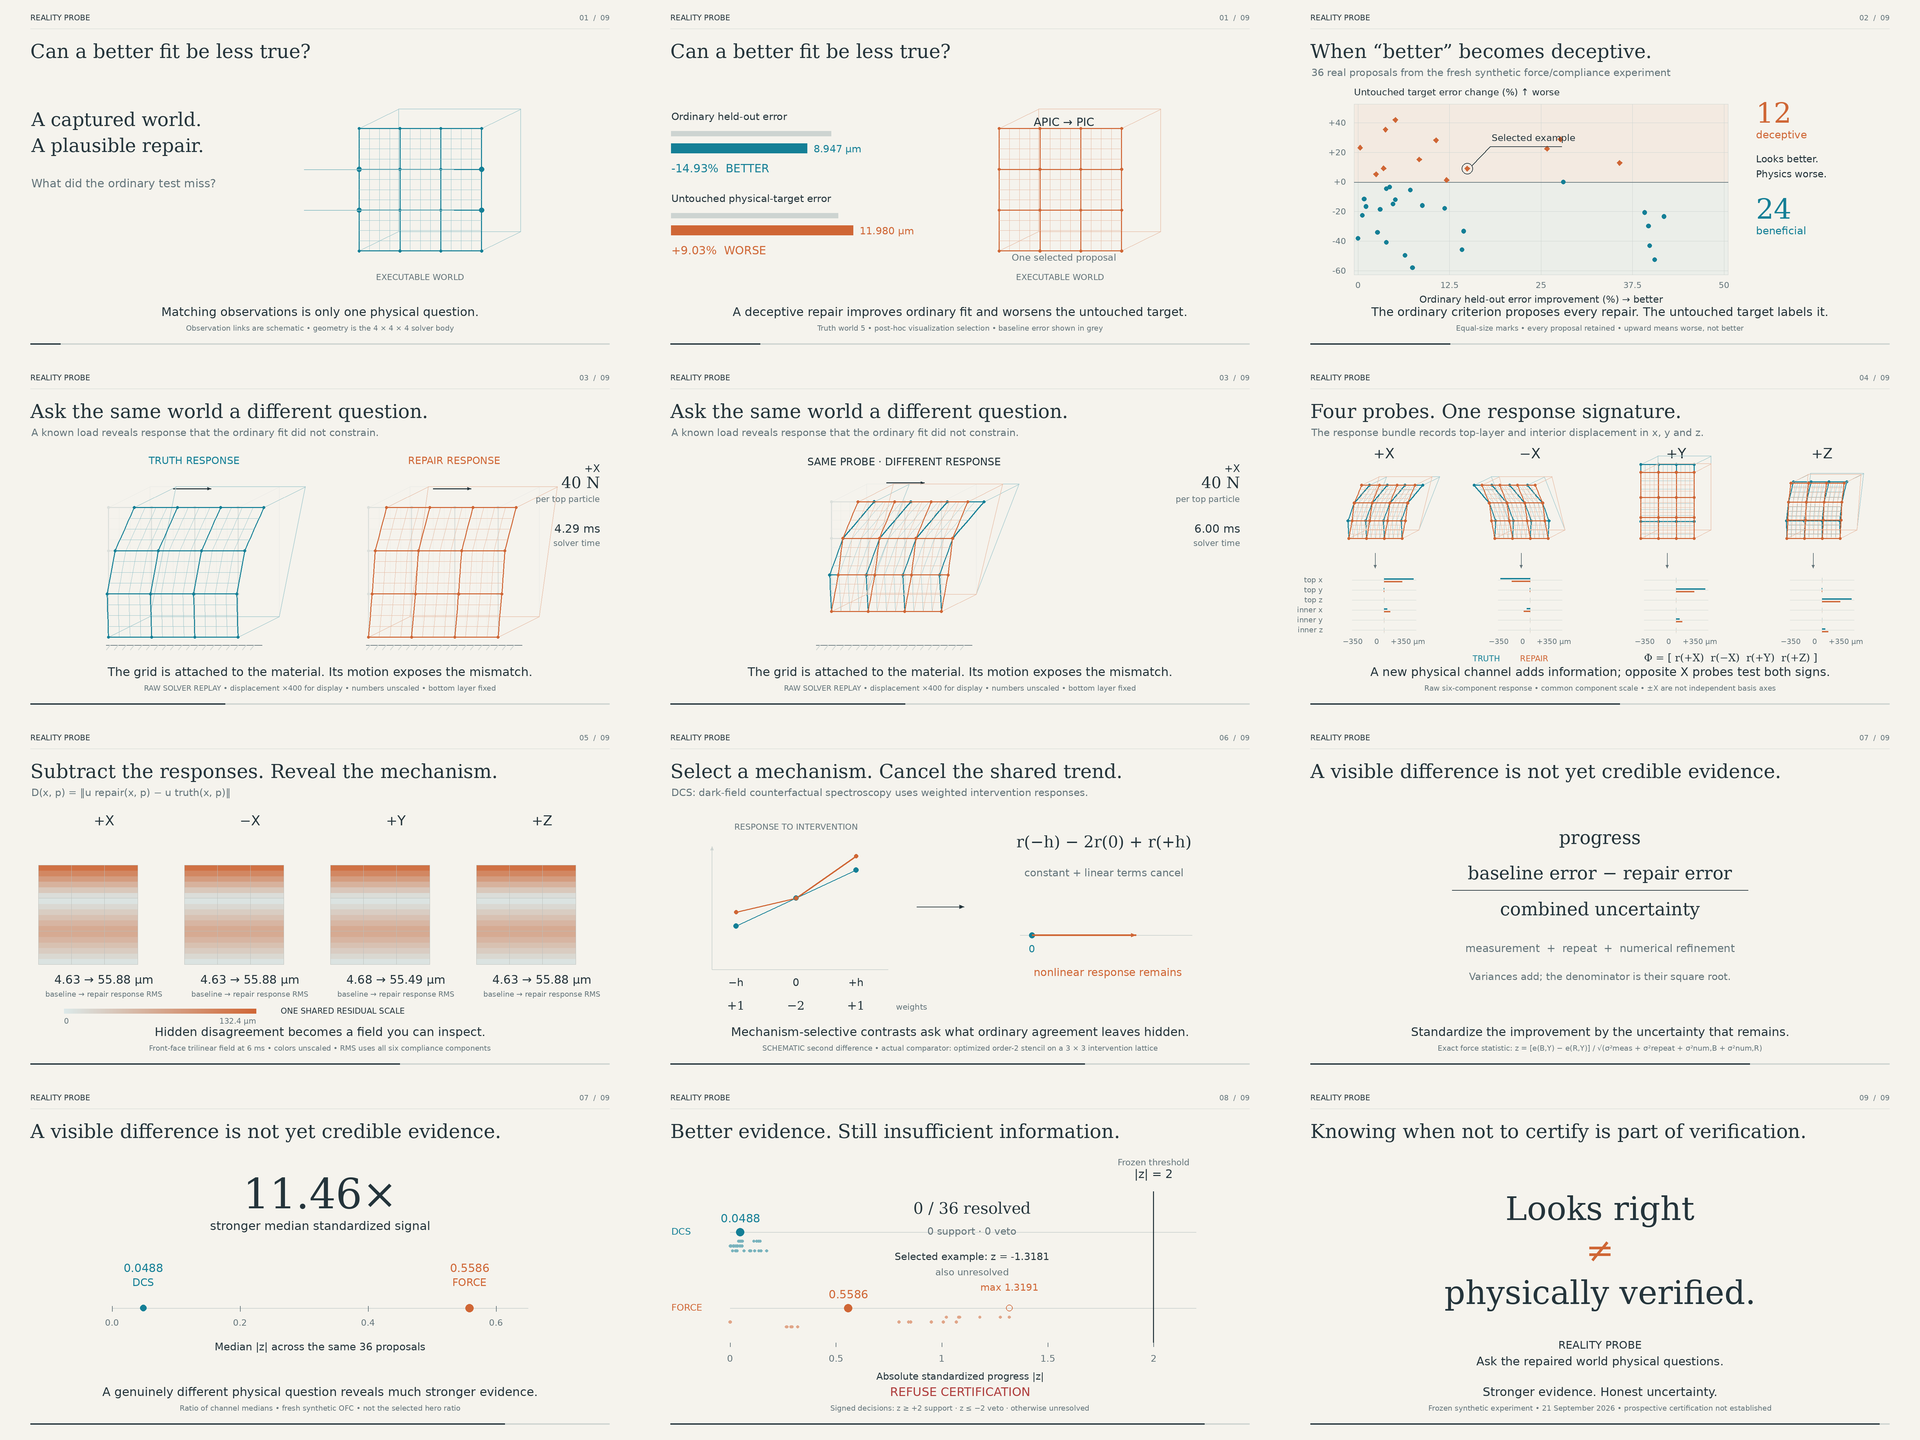
\includegraphics[width=\textwidth]{../docs/readme_assets/storyboard.png}
\caption{Reality Probe at a glance, composed from frozen result panels. A candidate repair can improve ordinary held-out fit while worsening an untouched physical target. The repair is then asked a different physical question, its motion response is compared with the reference response, mechanism-level residuals are exposed, and the evidence is standardized. The displayed case is post hoc for visualization; the 11.46$\times$ signal gain and 0/36 resolved coverage are aggregate fresh synthetic force-compliance results.}
\label{fig:overview}
\end{figure*}

\begin{figure}
\centering
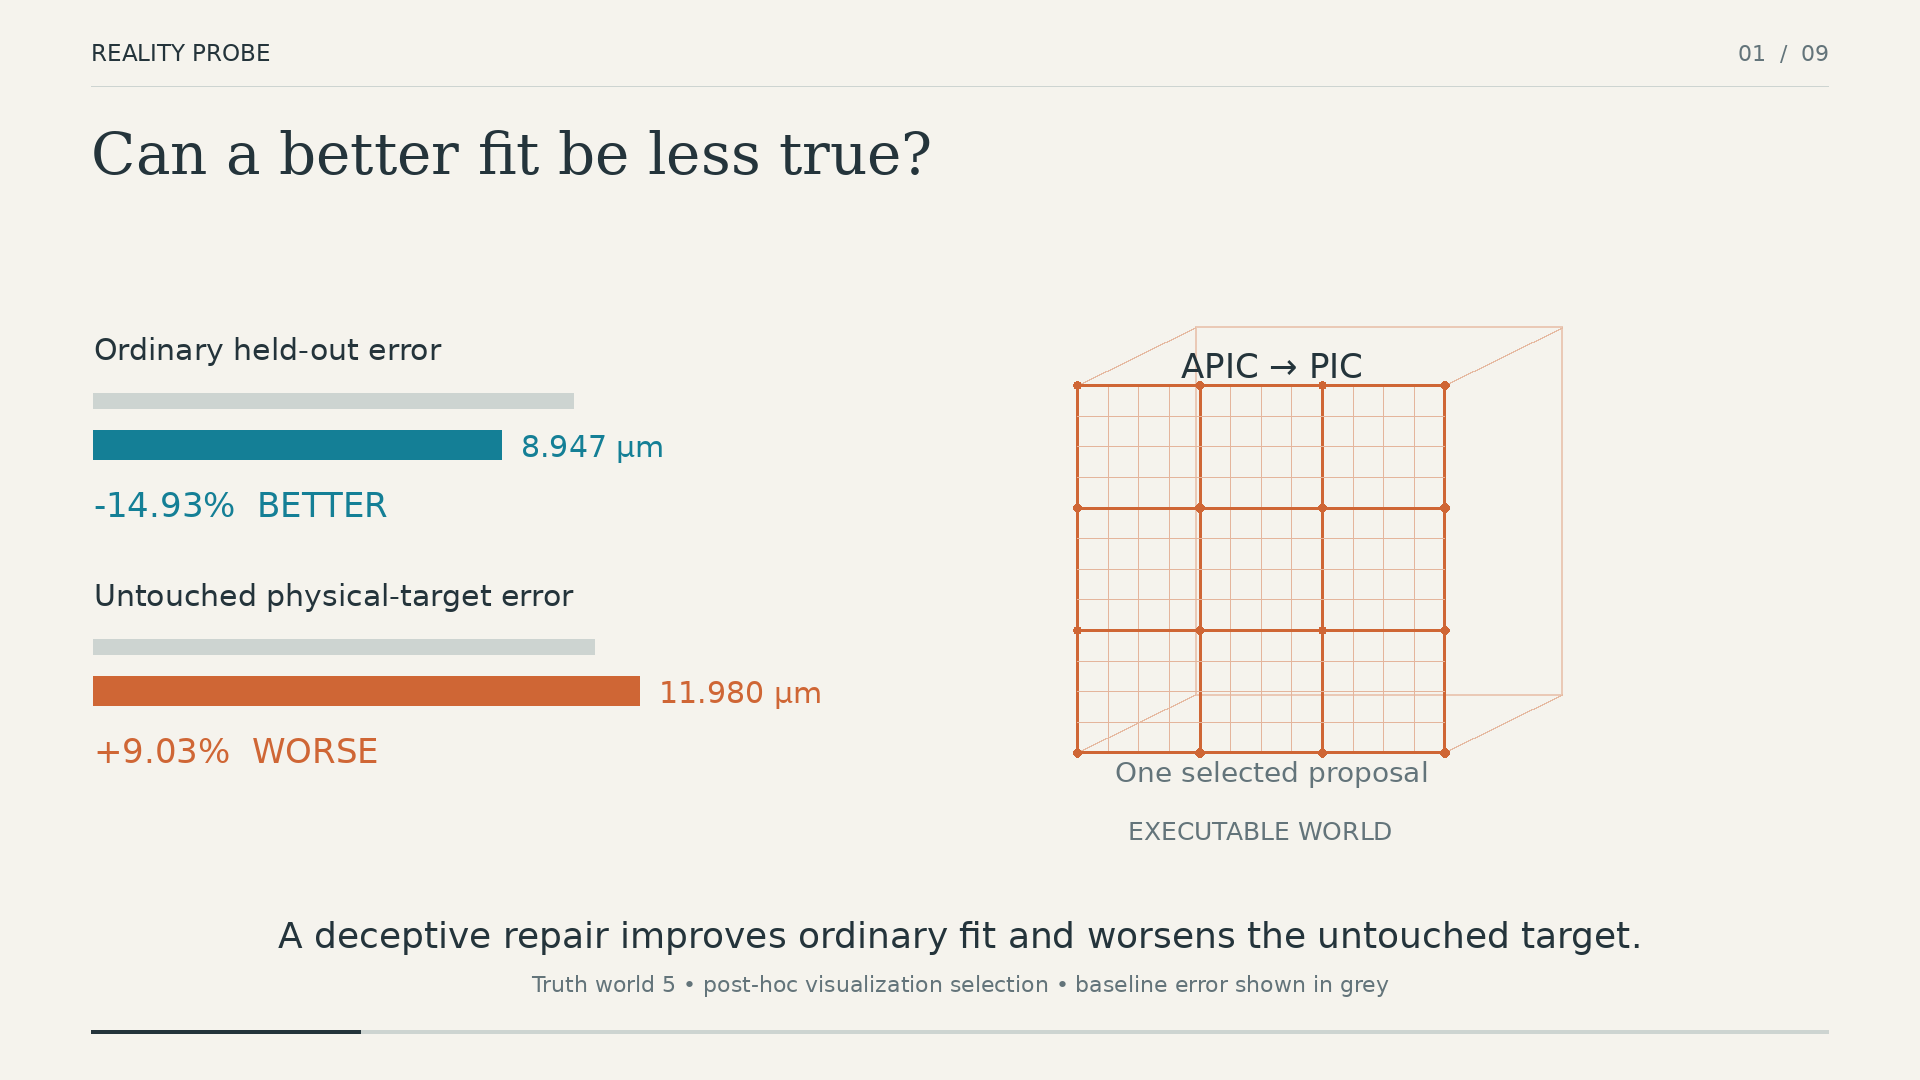
\includegraphics[width=\linewidth]{../docs/readme_assets/02_deceptive_repair.png}
\caption{Selected deceptive repair from the frozen fresh synthetic force-compliance population. Ordinary held-out error improves by 14.93\%, while untouched physical-target error worsens by 9.03\%. The selected case is illustrative only and does not affect aggregate statistics or decision thresholds.}
\label{fig:deceptive-repair}
\end{figure}

Reality Probe turns approval of such a rewrite into an explicit evidence transaction. Proposal generation uses fitting data and ordinary held-out observations. Verification begins after the proposal is fixed and uses a separately reserved physical channel. The verifier compares the baseline and candidate against that evidence, carries measurement, repeat, and numerical uncertainty, and returns SUPPORT, VETO, or UNRESOLVED. SUPPORT indicates that the candidate improves the reserved physical error by at least the frozen evidence margin; VETO indicates the opposite; UNRESOLVED records that the available experiment does not separate the two strongly enough.

Dark-Field Counterfactual Spectroscopy (DCS) is one probe tested inside this contract. DCS forms signed combinations of intervention responses so that lower-order common behavior cancels and higher-order disagreement becomes easier to observe. The cancellation machinery comes from classical finite-difference and inclusion--exclusion constructions. The scientific question here is empirical: does that type of contrast provide enough information to verify a captured-world rewrite under frozen uncertainty and decision rules?

The answer is mixed, and the experimental program is designed to preserve that fact. DCS passes a constructed positive control, then fails to produce resolved evidence in frozen truth-world validation, witness-space refinement, and a pair-specific repair-veto population. Matched raw, Fisher-style, and maximum-motion comparators also remain unresolved in the repair-veto stage. A new known-force compliance channel is then frozen before execution. It raises median standardized evidence magnitude by 11.46$\times$ on fresh synthetic truth worlds but still leaves all 36 proposals below the decision magnitude.

Measured video provides both a positive result and a boundary case. On 10 fresh IRIS \texttt{pendulum\_90} videos, the finite-amplitude period probe makes 90/110 controlled decisions correctly, compared with 40/110 for the small-angle diagnostic baseline, with all 10 placebo cases left UNRESOLVED. The 110 rows are nested controlled cases across 10 videos; they are not 110 independent physical experiments. A separately frozen IRIS free-fall replication then passes low-level quality checks on all five validation videos but fails physical recovery with 111.7\% median acceleration relative error. That validation split is retained as a failure, and the designated final split remains unopened.

The paper contributes four separable pieces of the overall argument:

\begin{enumerate}
\def\labelenumi{\arabic{enumi}.}
\item
  \textbf{A rewrite-level verification contract.} Reality Probe defines how proposal evidence, reserved physical evidence, uncertainty, and a three-way SUPPORT/VETO/UNRESOLVED decision are recorded before a captured-world rewrite is committed.
\item
  \textbf{A falsification-based information study.} Frozen synthetic stages show that a mathematically valid mechanism-sensitive probe can still be information-poor, and that a known-force channel can increase the evidence scale by 11.46$\times$ without reaching the same fixed decision boundary.
\item
  \textbf{A locked measured-video success case.} On 10 fresh IRIS pendulum videos, the finite-amplitude probe achieves 90/110 correct nested controlled decisions, compared with 40/110 for the matched small-angle diagnostic baseline, while preserving all 10 placebo abstentions.
\item
  \textbf{A preserved cross-domain failure.} The frozen IRIS free-fall validation passes tracking quality on 5/5 videos but fails the physical recovery gate. Post-validation rescue analyses do not produce a robust target-free estimator, so the lane is retired without opening its final split.
\end{enumerate}

The central question throughout the paper is therefore concrete: \emph{what physical evidence is sufficient to approve this rewrite?} The experiments show that the answer depends on the information carried by the verification channel, and that an unresolved result can be the correct endpoint of a well-functioning verifier.

\section{Related Work}\label{related-work}

\subsection{Physics-aware scene representations and inverse physics}\label{physics-aware-scene-representations-and-inverse-physics}

PAC-NeRF couples continuum simulation to a neural radiance field so that geometry and physical parameters can be estimated jointly from multi-view video \citep{li2023pacnerf}. PhysGaussian brings Material Point Method (MPM) dynamics into 3D Gaussian primitives \citep{xie2024physgaussian}. Subsequent systems extend physics-aware visual representations toward material initialization and refinement, interaction synthesis, and monocular or multi-material inverse physics \citep{zhang2024physdreamer,liu2025physflow,rho2026monophysics,wada2026mphygs}. These methods establish the proposal side of our setting: a captured representation can support simulation and physical parameter inference. Reality Probe begins after such a proposal exists and asks how a particular rewrite should be verified before commit.

Differentiable simulators such as ChainQueen and DiffTaichi provide infrastructure for gradient-based physical optimization \citep{hu2019chainqueen,hu2020difftaichi}. Our implementation similarly uses finite differences, adjoint sensitivity, APIC/MPM replay, and material calibration. These components support the experiments but are not presented as new simulation algorithms.

\subsection{Identifiability and experiment design}\label{identifiability-and-experimental-design}

Physical inference is limited by what the observations can distinguish. Structural identifiability formalizes whether model parameters are recoverable from a given observation process, and recent work studies such conditions directly from video for classes of dynamical systems \citep{wang2026identifiability}. IRIS provides controlled real videos for evaluating parameter accuracy, identifiability, extrapolation, and governing-equation recovery \citep{khanbayov2026iris}. In mechanics, optimal experiment design uses sensitivity, Jacobian conditioning, and Fisher-information ideas to choose loading conditions that separate candidate models \citep{asadi2025oed}.

Reality Probe does not introduce a new identifiability theory or experiment-design criterion. It uses the same information question at the level of a proposed rewrite: after the candidate is fixed, does the reserved experiment separate it from the baseline by enough margin to justify a decision? The frozen unresolved outcomes in our experiments are therefore evidence about the available channel, not merely failed optimization runs.

\subsection{Simulation credibility and measured physical fidelity}\label{simulation-credibility-and-measured-physical-fidelity}

Verification, validation, uncertainty quantification, and intended-use credibility are established parts of computational modeling \citep{oberkampf2007pcmm}. Digital-twin research also considers how simulated counterfactuals should be validated \citep{laudy2026digitaltwin}. Reality Probe adopts that credibility discipline for an individual physical rewrite in a persistent captured world. Its scope is narrower than general model certification: the system records whether a specific candidate is supported, vetoed, or left unresolved by a reserved physical channel.

GAUGE provides measurement-grounded tests of physical fidelity across simulation engines and video world models for rigid, cable, textile, and volumetric-deformation tasks \citep{wang2026gauge}. We use two GAUGE evidence classes and keep them separate. The foam-shearing study is retrospective: ordinary and marker channels prefer one model, while a longitudinal mechanism channel prefers another in 9/10 held-out repeats. A later repository-frozen validation lane uses previously untouched stretching and compression repeats 5--7. Across 12 measured worlds, the temporal annihilating witness makes 0/12 correct SUPPORT decisions and 0/12 correct VETO decisions, while all 12 placebo cases remain UNRESOLVED. Saved-output forensics show correct raw truth ordering but a signal only about 0.28\% of repeat variability and 11.8\% of nominal-versus-refined numerical discrepancy. We therefore treat that lane as an information-limit result and leave repeats 8--10 unopened.

\subsection{Measured deformable tracking}\label{measured-deformable-tracking}

Sequence C2 from the DOT deformable tracking dataset provides measured 3D correspondences through invisible markers \citep{li2025dot}. It is useful for exercising the captured-world reconstruction and fitting pipeline on measured deformable motion. DOT does not provide the stress-free state, applied loads, thickness, mass, or constitutive ground truth needed to identify a unique cloth material. We therefore report fitted parameters from this check as model-conditioned effective quantities and keep them outside the main physical-verification claim.

\section{Problem Formulation}\label{problem-formulation}

Let \(M\) denote an executable captured world. A baseline physical realization \(R_0\) has already been fitted, and an optimizer proposes a candidate realization \(R_1\). The experiments assign observations to three roles. \emph{Fitting evidence} may change the model or generate the proposal. \emph{Ordinary held-out evidence} measures generalization within the same observation family without fitting on those samples. \emph{Reserved physical evidence} is withheld until the candidate has been fixed and is used only for verification.

Let \(L_{\mathrm{obs}}(R)\) be the scalar ordinary held-out loss for realization \(R\), with lower values indicating better agreement. Let \(L_{\mathrm{target}}(R)\) be the error on an untouched physical target, again with lower values preferred. We call \(R_1\) a deceptive rewrite when

\[
L_{\mathrm{obs}}(R_1) < L_{\mathrm{obs}}(R_0)
\quad\text{and}\quad
L_{\mathrm{target}}(R_1) > L_{\mathrm{target}}(R_0).
\]

The definition identifies an evidence mismatch. It does not prescribe its cause. Model-form error, compensating parameters, boundary assumptions, transfer choices, or numerical effects can all produce a candidate that fits one observation family better and behaves worse under another physical test.

For verification, let \(Y\) denote the reserved physical evidence and \(e(R,Y)\) the error between realization \(R\) and that evidence. The error may be measured in different physical units in different experiments; the uncertainty scale \(\sigma\) uses the same units as the numerator. We define the signed standardized progress score

\[
z =
\frac{e(R_0,Y)-e(R_1,Y)}
     {\sigma}.
\]

A positive score means that the candidate is closer to the reserved evidence than the baseline. A negative score means that the candidate is worse. Dividing by \(\sigma\) expresses that improvement or degradation relative to the uncertainty carried by the experiment. The score is an operational standardized evidence measure; we do not interpret it as a Gaussian statistical \(z\)-test.

The frozen decision rule is

\[
z \geq 2 \Rightarrow \mathrm{SUPPORT},
\qquad
z \leq -2 \Rightarrow \mathrm{VETO},
\qquad
|z|<2 \Rightarrow \mathrm{UNRESOLVED}.
\]

The magnitude 2 is a repository-frozen decision reference for these experiments. It is neither a physical constant nor a universal credibility threshold. Keeping it fixed after data access is essential to the interpretation of the negative results: weak evidence remains weak rather than being converted into a decision by post-hoc threshold changes.

\section{Reality Probe}\label{reality-probe}

\subsection{Captured-world rewrite transaction}\label{captured-world-rewrite-and-verification-pipeline}

Reality Probe keeps proposal generation and verification sequential. A captured-world bundle stores appearance-linked state, particle state, observations, uncertainty sidecars, and provenance. The fitting split calibrates the baseline and may generate a candidate rewrite. Ordinary held-out observations measure whether that candidate generalizes within the proposal evidence family. Once the candidate is fixed, the verifier evaluates a separately reserved physical channel and records the resulting evidence score and decision.

The evidence layer has three outcomes. SUPPORT means the candidate clears the positive decision margin; VETO means it clears the negative margin; UNRESOLVED means the measured separation is too small relative to the uncertainty scale. The storage transaction is binary even though the scientific decision is ternary. SUPPORT may permit a verified commit. VETO and UNRESOLVED both leave the candidate uncommitted, but the evidence record preserves the difference between contradiction and insufficient information.

This ordering protects the role of the reserved evidence. If the verification channel is consulted while the candidate is still being selected, it becomes part of the proposal objective and no longer tests the proposed rewrite on held-out physical information.

The research implementation is written in C++20 and includes nonlinear MPM replay, APIC/PIC transfer variants, finite-difference and adjoint influence paths, deterministic experiment drivers, frozen JSON/CSV result ledgers, and SHA-256-indexed evidence packages. Metal and Vulkan render paths provide system integration and presentation. The quantitative claims reported here come from the recorded experiment outputs rather than from renderer-specific behavior.

\subsection{Dark-Field Counterfactual Spectroscopy}\label{dark-field-counterfactual-spectroscopy}

For a physical model \(M\) and intervention vector \(u\), let \(F_M(u)\) denote the observable response. Depending on the experiment, that response may contain displacement, motion, or another measured physical quantity. DCS evaluates several interventions \(u_i\) and combines their responses with signed weights \(w_i\):

\[
\mathcal{D}_{\mu}[F_M]
=
\sum_i w_i F_M(u_i).
\]

The signed measure \(\mu=\{(u_i,w_i)\}\) is chosen so that lower-order response terms cancel. For a declared cancellation order \(k\), the weights satisfy

\[
r_\alpha
=
\sum_i w_i u_i^\alpha
\approx 0,
\qquad
|\alpha|<k.
\]

Here \(\alpha\) is a multi-index that identifies a monomial in the intervention coordinates, and \(|\alpha|\) is its total degree. Small \(r_\alpha\) means that the stencil nearly annihilates that lower-order term. The implementation enumerates the required monomials and checks the largest residual against a tolerance, so the cancellation property is verified for each synthesized stencil.

A one-dimensional order-2 example is

\begin{equation}\label{eq:second}
F(+a)+F(-a)-2F(0),
\end{equation}

where \(a\) is the intervention amplitude. The constant terms cancel because the weights sum to zero, and a response that is linear in \(a\) also cancels between \(+a\) and \(-a\). The remaining value therefore emphasizes curvature and other higher-order response. Equation~\ref{eq:second} is only an intuition-building example; the reported order-2 experiments synthesize their comparator on a \(3\times3\) intervention lattice.

For finite-amplitude interactions, the implementation also evaluates the Boolean-lattice M\"obius contrast

\[
\kappa(S)
=
\sum_{T\subseteq S}
(-1)^{|S|-|T|}F(T),
\]

where \(S\) is a set of simultaneously active intervention factors and \(T\) enumerates its subsets. The alternating sum removes contributions already explained by lower-order subsets and leaves the finite-amplitude interaction associated with the full set. We use \(\kappa(S)\) as an interaction statistic and make no claim that this classical construction is a new mixed-derivative result.

\subsection{Uncertainty and standardized separation}\label{uncertainty-and-standardized-separation}

The verifier keeps three uncertainty sources explicit. Measurement uncertainty describes error in the observed physical quantity. Repeat uncertainty measures variation across repeated acquisitions or trials. Numerical uncertainty measures sensitivity to solver resolution or discretization. For a signed DCS stencil, independent measurement and repeat variances propagate with the squared weight gain \(\sum_i w_i^2\). Numerical errors can be correlated across intervention points, so D3 also measures numerical change directly in witness space by evaluating the same signed witness at nominal and refined solver resolution.

Candidate disagreement is evaluated as a standardized separation: a physical error difference divided by the combined uncertainty scale for that comparison. This normalization answers a practical question that raw error cannot: is the observed improvement large relative to the uncertainty of the experiment?

Active stencil synthesis searches within the nullspace of the lower-moment constraints. Candidate disagreement is projected into that nullspace, and the implementation evaluates a deterministic set of projected directions before retaining the strongest admissible witness. Because the resulting maximin search is non-convex, we treat this synthesis as a deterministic heuristic. The experiments evaluate whether the witnesses it produces are useful; they do not assume global optimality.

\subsection{Known-force compliance as a different information channel}\label{known-force-compliance-as-orthogonal-information}

D4V leaves every repair unresolved under the tested kinematic verification channels. We therefore freeze a new experiment that changes the physical information supplied to the verifier. Proposal generation remains unchanged. After each candidate is fixed, a known external force is applied and the resulting compliance is measured.

The fresh population contains six APIC truth worlds. Young's modulus takes values in \(\{14125,16625,18125\}\) Pa, Poisson ratio in \(\{0.22,0.32\}\), and the truth timestep is \(2.5\times10^{-5}\) s. Candidate families are fixed before execution. The bottom particle layer is kinematically fixed and gravity is disabled. Every top-layer particle receives a 40 N load in four separate directions: \(+x\), \(-x\), \(+y\), and \(+z\). For each load we record mean top-layer and interior-layer displacement along three axes, giving a six-component response bundle per force direction.

Numerical uncertainty is the root-mean-square difference between nominal and half-timestep candidate response bundles. Measurement and repeat scales are each frozen at \(2\times10^{-5}\) m per component. If \(B\) denotes the baseline, \(R\) the candidate, and \(Y\) the truth response, the force-compliance score is

\[
z_{\mathrm{force}}
=
\frac{e(B,Y)-e(R,Y)}
{\sqrt{
\sigma_{\mathrm{meas}}^2+
\sigma_{\mathrm{repeat}}^2+
\sigma_{\mathrm{num},B}^2+
\sigma_{\mathrm{num},R}^2
}}.
\]

The numerator is positive when the candidate matches the truth response better than the baseline. The denominator combines the frozen measurement and repeat scales with baseline and candidate numerical uncertainty, all in compatible displacement-error units. The force channel and the fresh DCS comparator use the same decision magnitude of 2. Force amplitude, directions, truth worlds, candidate grid, and threshold are fixed before execution.

\begin{figure}
\centering
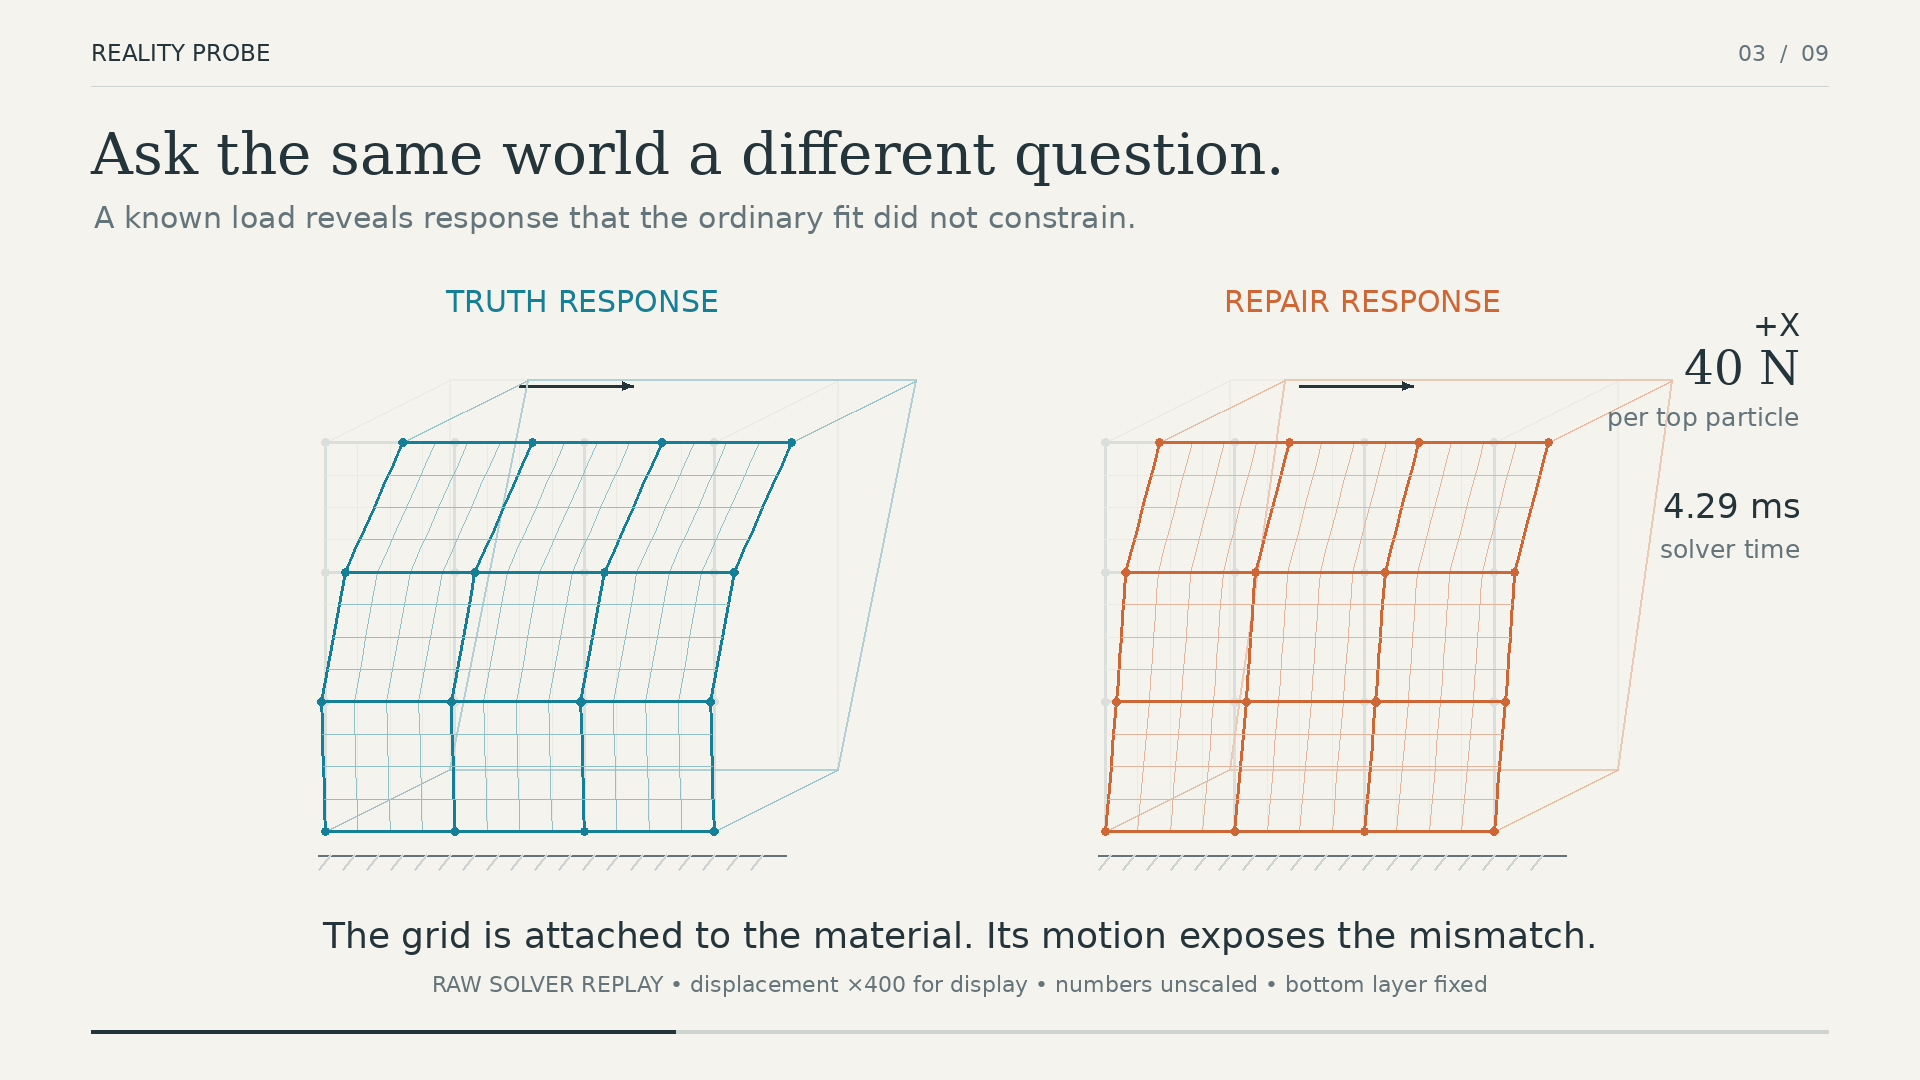
\includegraphics[width=\linewidth]{../docs/readme_assets/04_same_probe.png}
\caption{The same controlled \(+x\) force probe applied to the truth and repaired worlds. Displayed deformation is magnified 400$\times$ for legibility; every reported quantitative result uses the unscaled displacement.}
\label{fig:same-probe}
\end{figure}

\begin{figure}
\centering
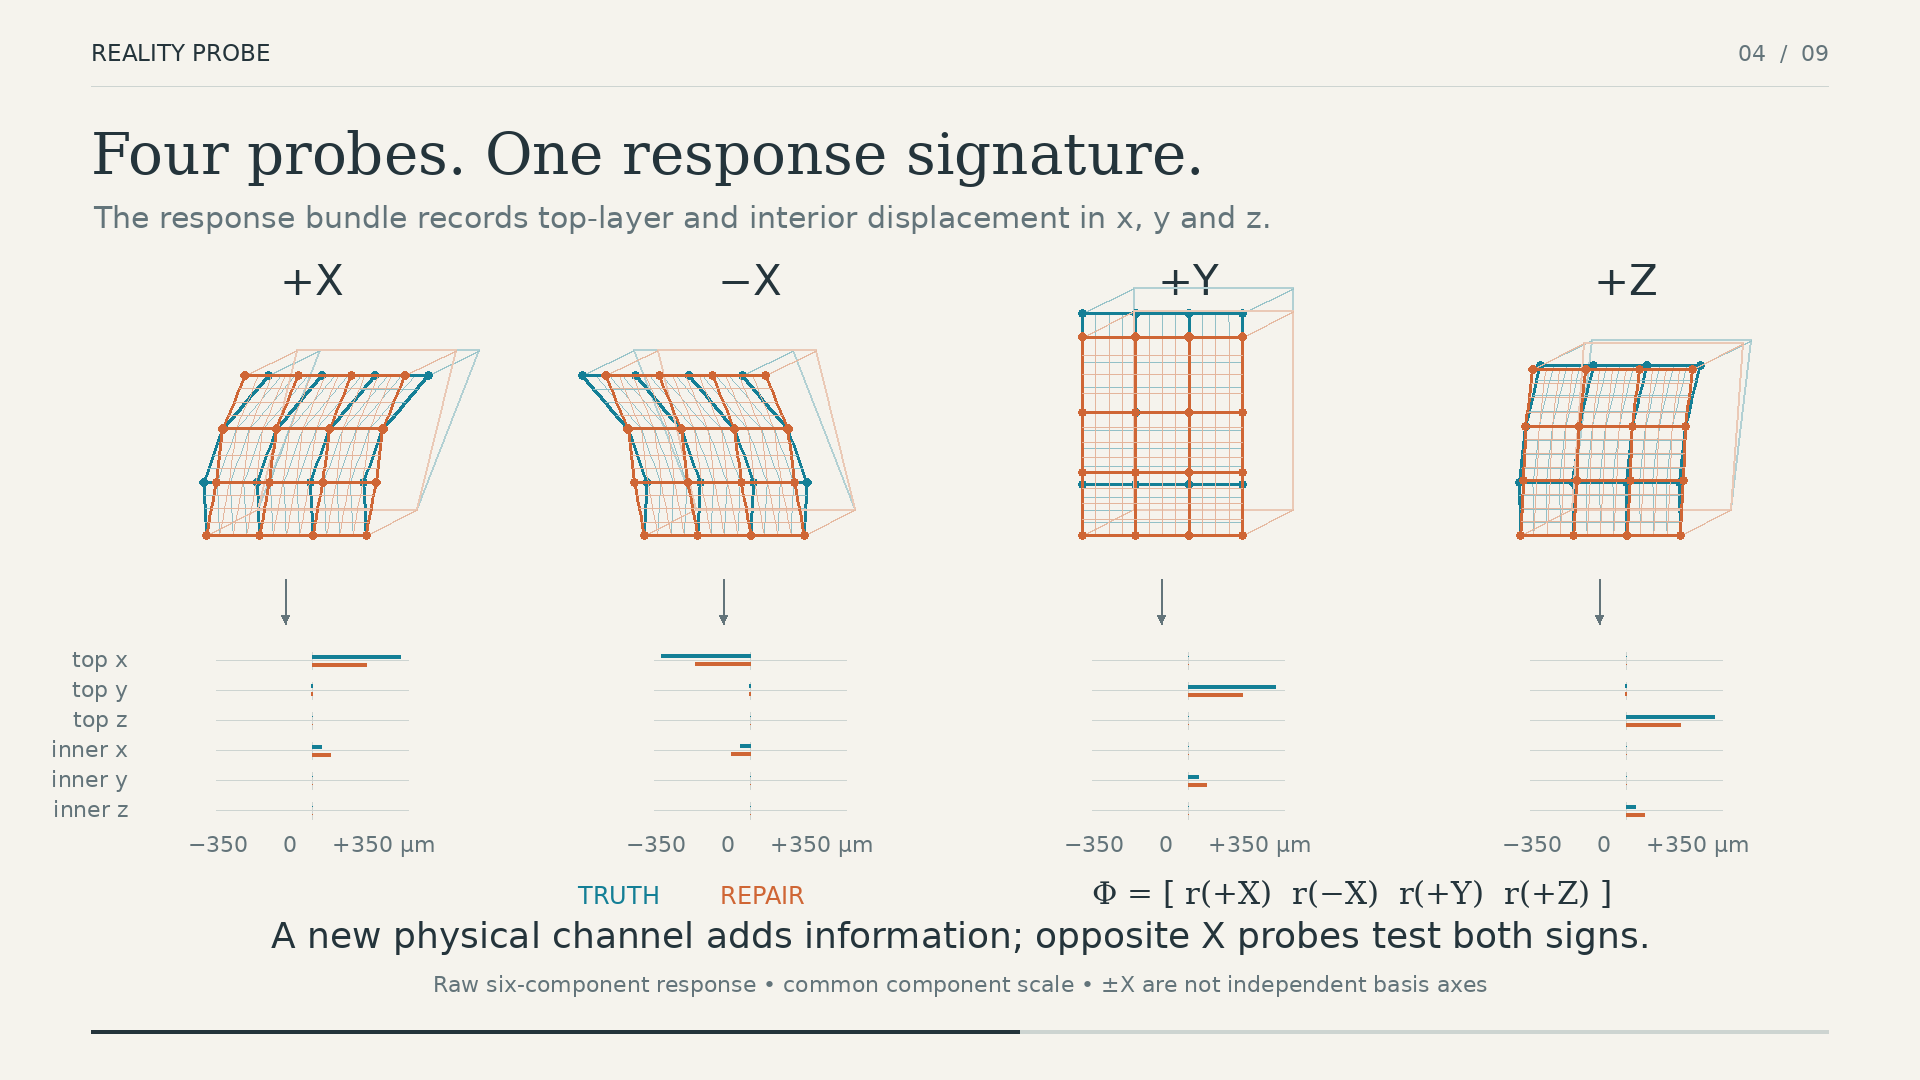
\includegraphics[width=\linewidth]{../docs/readme_assets/06_fingerprint.png}
\caption{Four-direction force-response fingerprint for the selected frozen case. The six-component response bundle records top-layer and interior displacement under \(+x\), \(-x\), \(+y\), and \(+z\) probes. Truth and candidate responses share one component scale.}
\label{fig:force-fingerprint}
\end{figure}

\begin{figure}
\centering
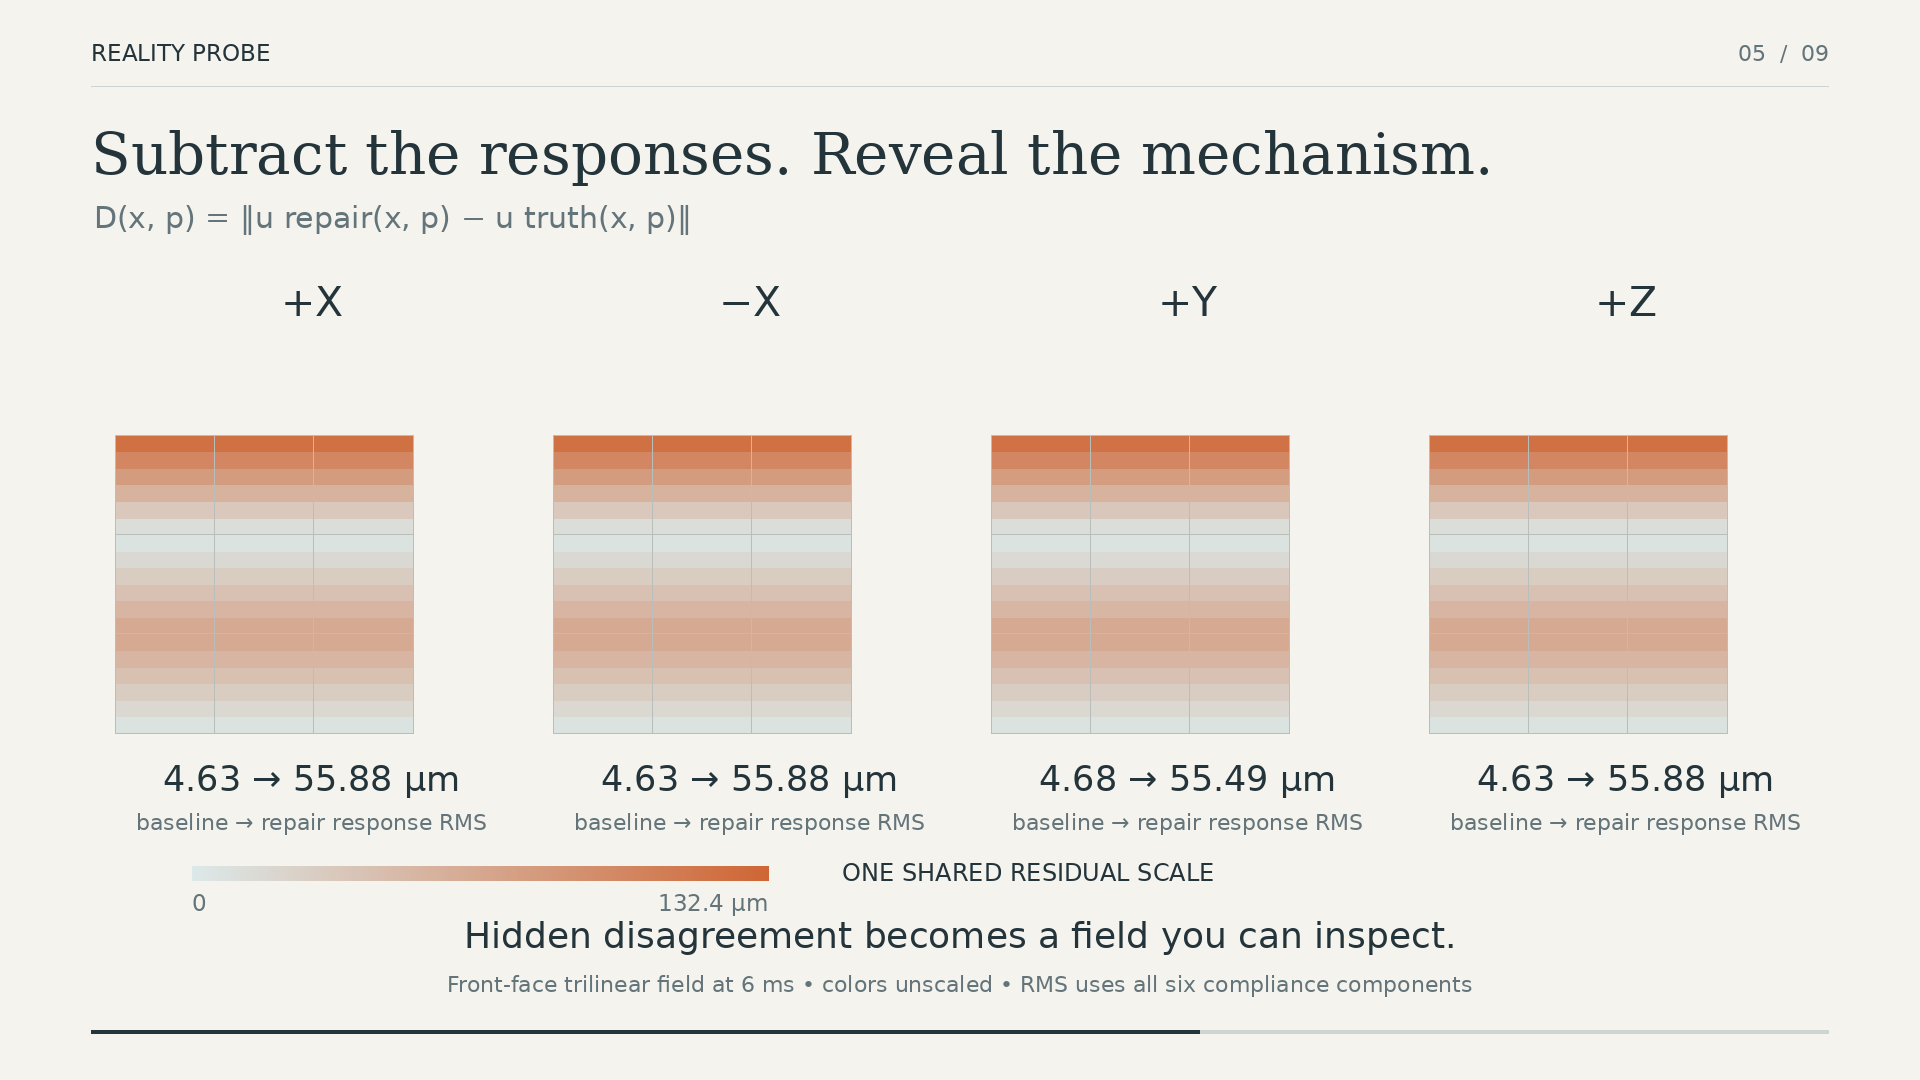
\includegraphics[width=\linewidth]{../docs/readme_assets/07_residual_field.png}
\caption{Solver-driven residual field for the same frozen visualization case. All four force directions share one residual scale. The field explains where the responses differ; it is not itself the DCS decision statistic.}
\label{fig:residual-field}
\end{figure}

\section{Experimental Program}\label{experimental-program}

The experiments are organized by evidence role because the same numerical outcome means different things depending on when the data were seen. Constructed controls test whether an implementation can express the intended behavior. Frozen validation tests a protocol after its choices have been fixed. Retrospective measured analyses diagnose already-observed behavior. Locked final tests use media reserved until the protocol has passed its earlier gates. Post-final analyses may probe robustness or alternative explanations, but they cannot replace the locked result.

Table~\ref{tab:stages} summarizes this evidence ladder. Here, resolved refers to the frozen SUPPORT/VETO rule. An unresolved experiment can still reveal how much information is missing or which source of uncertainty dominates.

\begin{table*}[t]
\centering
\caption{Experimental stages and evidence classes. Detailed numerical outcomes are reported in Sec.~\ref{results-and-analysis}.}
\label{tab:stages}
\begin{tabularx}{\textwidth}{l l r X}
\toprule
Stage & Evidence class & Population & Purpose \\
\midrule
D1 & constructed synthetic control & 64 repairs & Check that the DCS path can reject a deliberately strong deceptive repair. \\
D2 & frozen synthetic validation & 16 truth worlds & Test whether the selected witness reaches the fixed decision margin on unseen truth worlds. \\
D3 & fresh synthetic refinement & 6 truth worlds & Separate numerical-resolution limits from physical observability limits. \\
D4V & frozen synthetic repair population & 36 repairs & Evaluate pair-specific verification on ordinary-improving proposals. \\
DOT C2 & measured engineering check & 225 correspondence points & Exercise capture, fitting, held-out replay, rewrite, verification, rollback, and visualization on measured deformable motion. \\
GAUGE shearing & retrospective measured analysis & 10 held-out repeats & Test whether ordinary and mechanism-sensitive channels can disagree on the same measured motion. \\
GAUGE validation & frozen measured validation & 12 measured worlds / 36 cases & Test directional SUPPORT/VETO coverage on previously untouched stretching/compression repeats. \\
OFC & fresh synthetic orthogonal channel & 36 repairs & Ask whether a different physical interrogation changes the evidence scale under the same decision magnitude. \\
IRIS pendulum & repository-locked measured final & 10 videos / 110 nested cases & Evaluate a matched physical observable on fresh final media. \\
IRIS free-fall & frozen measured validation & 5 validation videos & Test transfer to a second equation family without retuning on validation. \\
\bottomrule
\end{tabularx}
\end{table*}

\subsection{Evidence surfaces and benchmark roles}\label{graphics-facing-benchmark-and-visual-evidence-coverage}

The quantitative evidence comes from frozen JSON/CSV ledgers and measured dataset adapters. Figures expose the physical consequences of those experiments but do not create a second source of quantitative truth. Table~\ref{tab:graphics-evidence} makes the role of each source explicit.

\begin{table*}[t]
\centering
\caption{Evidence coverage. Public measured benchmarks are separated from controlled synthetic partitions and visualization-only geometry.}
\label{tab:graphics-evidence}
\begin{tabularx}{\textwidth}{l l X X}
\toprule
Source & Evidence class & What it contributes & Claim boundary \\
\midrule
DOT C2 \citep{li2025dot} & public measured trajectories & End-to-end captured-world ingestion, fit/held-out replay, local rewrite, verification, rollback, and measured-motion visualization. & Stress-free state, loads, thickness, mass, and constitutive ground truth are absent; fitted material values remain model-conditioned. \\
GAUGE \citep{wang2026gauge} & public measured benchmark & Retrospective shearing contradiction and a separately frozen stretching/compression validation lane. & The shearing study is retrospective; the validation lane is a failed validation-stage result, not final confirmation. \\
IRIS \citep{khanbayov2026iris} & public measured benchmark & Locked pendulum confirmation and a separately frozen free-fall validation attempt. & The 110 pendulum cases are nested in 10 videos; the free-fall lane fails validation and its final split remains unopened. \\
D2/D3/D4V + OFC & controlled synthetic & Known-ground-truth falsification, pair-specific rewrite evaluation, and a frozen change of physical evidence channel. & Controlled evidence, not measured-world force-sensor validation. \\
Stanford Bunny visual suite & visualization carrier & Solver-driven deformation, force direction, mechanism fingerprints, and residual fields. & Visualization only; it contributes no benchmark result. \\
\bottomrule
\end{tabularx}
\end{table*}

The deceptive-repair, same-probe, force-fingerprint, residual-field, signal-gain, and information-limit panels are generated from committed solver trajectories or frozen result ledgers. Display magnification is disclosed where used; numerical values are computed from the unscaled simulation outputs.

\subsection{Synthetic falsification ladder}\label{synthetic-falsification-ladder}

\paragraph{D1: constructed control.}
D1 deliberately builds a strong deceptive-repair signal. Its purpose is implementation sanity: if the DCS path cannot reject these 64 constructed cases, later failures are uninterpretable.

\paragraph{D2: frozen validation.}
Discovery compares raw maximin, Fisher/Jacobian selection, a same-cost raw bundle, maximum motion, DCS order-2 maximin, and random selection. After the discovery choice is fixed, D2 evaluates 16 unseen synthetic truth worlds under the frozen decision magnitude.

\paragraph{D3: witness-space refinement.}
D3 uses six fresh truth worlds to test a specific alternative explanation for weak D2 evidence: solver discretization or cancellation order may be hiding an otherwise useful distinction. The same signed witness is evaluated at nominal and refined resolution, and adaptive selection may choose order 2 or 3.

\paragraph{D4V: pair-specific rewrite verification.}
D4V begins with 36 proposals that have already improved ordinary held-out error. The untouched physical target labels 14 as deceptive and 22 as beneficial. DCS is compared with raw-bundle, pair-specific raw, Fisher, and maximum-motion verification under the inherited \(|z|\ge2\) rule.

\begin{table}[t]
\centering
\caption{Ordinary-improving synthetic proposal populations. D4V and the fresh OFC population are separate partitions and are not pooled.}
\label{tab:populations}
\begin{tabular}{lrrr}
\toprule
Population & Deceptive & Beneficial & Resolved at \(|z|\ge2\) \\
\midrule
D4V & 14 & 22 & 0/36 \\
Fresh OFC & 12 & 24 & 0/36 \\
\bottomrule
\end{tabular}
\end{table}

\subsection{Measured engineering and GAUGE protocols}\label{measured-engineering-and-gauge-protocols}

The DOT C2 check uses measured 3D correspondences to exercise the full captured-world path. The importer keeps measured trajectories separate from explicit proxies for rest state, density, thickness, mass, Gaussian photometry, and uncertainty. Calibration uses only the fit split, followed by held-out replay and a local material rewrite. Because C2 does not provide constitutive ground truth, the fitted material parameters are interpreted only as effective parameters of the chosen model.

\begin{table}[t]
\centering
\caption{DOT C2 measured-source engineering check. The material parameters are model-conditioned effective values, not material ground truth.}
\label{tab:dot-c2}
\begin{tabularx}{\linewidth}{@{}>{\raggedright\arraybackslash}X >{\raggedleft\arraybackslash}p{0.47\linewidth}@{}}
\toprule
Quantity & Result \\
\midrule
Measured correspondence points & 225 \\
Trajectory observations (fit / held-out) & 675 (585 / 90) \\
Effective \(E,\nu\) & 7.5 kPa, 0.45 \\
Dynamic RMS (fit / held-out) & 4.391 / 4.417 mm \\
Adaptive candidate set & 182/225 particles; 94.80\% abs. gradient \\
Rewrite verification & nonlinear pass; oracle fail; rollback \\
\bottomrule
\end{tabularx}
\end{table}

\begin{figure}[t]
\centering
\resizebox{0.92\linewidth}{!}{% Auto-generated from the successful DOT C2 measured-source CI artifact.
% Source: build/dot-c2/calibration/selected_samples.csv, validation split, t=0.166667 s.
% Coordinates are plotted at one common x/y metric scale; residual segments are not magnified.
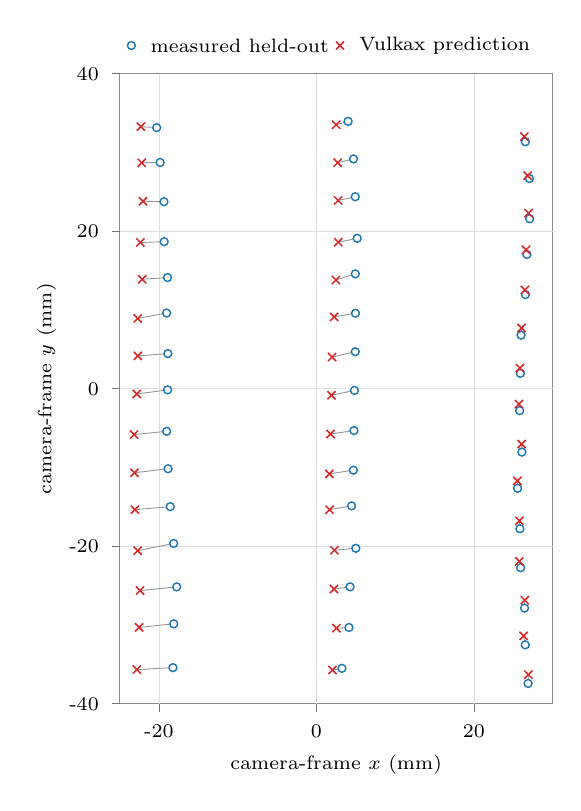
\begin{tikzpicture}[x=1cm,y=1cm]
  \definecolor{dotmeasured}{RGB}{31,119,180}
  \definecolor{dotpredicted}{RGB}{214,39,40}
  \draw[black!45,line width=0.35pt] (0,0) rectangle (5.500,8.000);
  \draw[black!12,line width=0.25pt] (0.500,0) -- (0.500,8.000);
  \draw[black!55,line width=0.3pt] (0.500,0) -- (0.500,-0.10);
  \node[font=\scriptsize,anchor=north] at (0.500,-0.14) {-20};
  \draw[black!12,line width=0.25pt] (2.500,0) -- (2.500,8.000);
  \draw[black!55,line width=0.3pt] (2.500,0) -- (2.500,-0.10);
  \node[font=\scriptsize,anchor=north] at (2.500,-0.14) {0};
  \draw[black!12,line width=0.25pt] (4.500,0) -- (4.500,8.000);
  \draw[black!55,line width=0.3pt] (4.500,0) -- (4.500,-0.10);
  \node[font=\scriptsize,anchor=north] at (4.500,-0.14) {20};
  \draw[black!55,line width=0.3pt] (0,0.000) -- (-0.10,0.000);
  \node[font=\scriptsize,anchor=east] at (-0.14,0.000) {-40};
  \draw[black!12,line width=0.25pt] (0,2.000) -- (5.500,2.000);
  \draw[black!55,line width=0.3pt] (0,2.000) -- (-0.10,2.000);
  \node[font=\scriptsize,anchor=east] at (-0.14,2.000) {-20};
  \draw[black!12,line width=0.25pt] (0,4.000) -- (5.500,4.000);
  \draw[black!55,line width=0.3pt] (0,4.000) -- (-0.10,4.000);
  \node[font=\scriptsize,anchor=east] at (-0.14,4.000) {0};
  \draw[black!12,line width=0.25pt] (0,6.000) -- (5.500,6.000);
  \draw[black!55,line width=0.3pt] (0,6.000) -- (-0.10,6.000);
  \node[font=\scriptsize,anchor=east] at (-0.14,6.000) {20};
  \draw[black!55,line width=0.3pt] (0,8.000) -- (-0.10,8.000);
  \node[font=\scriptsize,anchor=east] at (-0.14,8.000) {40};
  \node[font=\scriptsize,anchor=north] at (2.750,-0.52) {camera-frame $x$ (mm)};
  \node[font=\scriptsize,rotate=90,anchor=south] at (-0.68,4.000) {camera-frame $y$ (mm)};
  \draw[black!42,line width=0.32pt] (0.6777,0.4588) -- (0.2189,0.4347);
  \draw[black!42,line width=0.32pt] (2.8242,0.4503) -- (2.7033,0.4289);
  \draw[black!42,line width=0.32pt] (5.1880,0.2578) -- (5.1911,0.3689);
  \draw[black!42,line width=0.32pt] (0.6878,1.0153) -- (0.2478,0.9708);
  \draw[black!42,line width=0.32pt] (2.9132,0.9690) -- (2.7539,0.9595);
  \draw[black!42,line width=0.32pt] (5.1518,0.7486) -- (5.1308,0.8628);
  \draw[black!42,line width=0.32pt] (0.7254,1.4843) -- (0.2605,1.4379);
  \draw[black!42,line width=0.32pt] (2.9269,1.4853) -- (2.7225,1.4575);
  \draw[black!42,line width=0.32pt] (5.1429,1.2153) -- (5.1458,1.3157);
  \draw[black!42,line width=0.32pt] (0.6868,2.0363) -- (0.2302,1.9444);
  \draw[black!42,line width=0.32pt] (3.0001,1.9747) -- (2.7277,1.9494);
  \draw[black!42,line width=0.32pt] (5.0940,1.7273) -- (5.0761,1.8087);
  \draw[black!42,line width=0.32pt] (0.6438,2.5029) -- (0.1942,2.4662);
  \draw[black!42,line width=0.32pt] (2.9460,2.5137) -- (2.6661,2.4649);
  \draw[black!42,line width=0.32pt] (5.0836,2.2231) -- (5.0779,2.3239);
  \draw[black!42,line width=0.32pt] (0.6158,2.9848) -- (0.1899,2.9342);
  \draw[black!42,line width=0.32pt] (2.9693,2.9665) -- (2.6642,2.9202);
  \draw[black!42,line width=0.32pt] (5.0544,2.7367) -- (5.0519,2.8304);
  \draw[black!42,line width=0.32pt] (0.5979,3.4598) -- (0.1842,3.4188);
  \draw[black!42,line width=0.32pt] (2.9764,3.4694) -- (2.6785,3.4258);
  \draw[black!42,line width=0.32pt] (5.1087,3.1961) -- (5.1057,3.2981);
  \draw[black!42,line width=0.32pt] (0.6100,3.9865) -- (0.2180,3.9343);
  \draw[black!42,line width=0.32pt] (2.9825,3.9794) -- (2.6919,3.9180);
  \draw[black!42,line width=0.32pt] (5.0813,3.7226) -- (5.0720,3.8062);
  \draw[black!42,line width=0.32pt] (0.6130,4.4469) -- (0.2327,4.4185);
  \draw[black!42,line width=0.32pt] (2.9928,4.4712) -- (2.6986,4.4034);
  \draw[black!42,line width=0.32pt] (5.0895,4.1969) -- (5.0840,4.2633);
  \draw[black!42,line width=0.32pt] (0.5973,4.9625) -- (0.2297,4.8933);
  \draw[black!42,line width=0.32pt] (2.9957,4.9600) -- (2.7246,4.9131);
  \draw[black!42,line width=0.32pt] (5.0986,4.6811) -- (5.1046,4.7728);
  \draw[black!42,line width=0.32pt] (0.6087,5.4129) -- (0.2868,5.3913);
  \draw[black!42,line width=0.32pt] (2.9936,5.4597) -- (2.7468,5.3819);
  \draw[black!42,line width=0.32pt] (5.1545,5.1964) -- (5.1486,5.2558);
  \draw[black!42,line width=0.32pt] (0.5664,5.8686) -- (0.2644,5.8581);
  \draw[black!42,line width=0.32pt] (3.0178,5.9113) -- (2.7778,5.8617);
  \draw[black!42,line width=0.32pt] (5.1725,5.7061) -- (5.1628,5.7654);
  \draw[black!42,line width=0.32pt] (0.5635,6.3761) -- (0.2975,6.3826);
  \draw[black!42,line width=0.32pt] (2.9927,6.4391) -- (2.7753,6.3919);
  \draw[black!42,line width=0.32pt] (5.2070,6.1600) -- (5.1931,6.2315);
  \draw[black!42,line width=0.32pt] (0.5147,6.8749) -- (0.2806,6.8707);
  \draw[black!42,line width=0.32pt] (2.9707,6.9204) -- (2.7698,6.8712);
  \draw[black!42,line width=0.32pt] (5.2049,6.6709) -- (5.1822,6.7074);
  \draw[black!42,line width=0.32pt] (0.4711,7.3174) -- (0.2703,7.3292);
  \draw[black!42,line width=0.32pt] (2.9025,7.3963) -- (2.7499,7.3533);
  \draw[black!42,line width=0.32pt] (5.1530,7.1382) -- (5.1404,7.2038);
  \draw[dotmeasured,line width=0.52pt,fill=white] (0.6777,0.4588) circle[radius=0.050];
  \draw[dotmeasured,line width=0.52pt,fill=white] (2.8242,0.4503) circle[radius=0.050];
  \draw[dotmeasured,line width=0.52pt,fill=white] (5.1880,0.2578) circle[radius=0.050];
  \draw[dotmeasured,line width=0.52pt,fill=white] (0.6878,1.0153) circle[radius=0.050];
  \draw[dotmeasured,line width=0.52pt,fill=white] (2.9132,0.9690) circle[radius=0.050];
  \draw[dotmeasured,line width=0.52pt,fill=white] (5.1518,0.7486) circle[radius=0.050];
  \draw[dotmeasured,line width=0.52pt,fill=white] (0.7254,1.4843) circle[radius=0.050];
  \draw[dotmeasured,line width=0.52pt,fill=white] (2.9269,1.4853) circle[radius=0.050];
  \draw[dotmeasured,line width=0.52pt,fill=white] (5.1429,1.2153) circle[radius=0.050];
  \draw[dotmeasured,line width=0.52pt,fill=white] (0.6868,2.0363) circle[radius=0.050];
  \draw[dotmeasured,line width=0.52pt,fill=white] (3.0001,1.9747) circle[radius=0.050];
  \draw[dotmeasured,line width=0.52pt,fill=white] (5.0940,1.7273) circle[radius=0.050];
  \draw[dotmeasured,line width=0.52pt,fill=white] (0.6438,2.5029) circle[radius=0.050];
  \draw[dotmeasured,line width=0.52pt,fill=white] (2.9460,2.5137) circle[radius=0.050];
  \draw[dotmeasured,line width=0.52pt,fill=white] (5.0836,2.2231) circle[radius=0.050];
  \draw[dotmeasured,line width=0.52pt,fill=white] (0.6158,2.9848) circle[radius=0.050];
  \draw[dotmeasured,line width=0.52pt,fill=white] (2.9693,2.9665) circle[radius=0.050];
  \draw[dotmeasured,line width=0.52pt,fill=white] (5.0544,2.7367) circle[radius=0.050];
  \draw[dotmeasured,line width=0.52pt,fill=white] (0.5979,3.4598) circle[radius=0.050];
  \draw[dotmeasured,line width=0.52pt,fill=white] (2.9764,3.4694) circle[radius=0.050];
  \draw[dotmeasured,line width=0.52pt,fill=white] (5.1087,3.1961) circle[radius=0.050];
  \draw[dotmeasured,line width=0.52pt,fill=white] (0.6100,3.9865) circle[radius=0.050];
  \draw[dotmeasured,line width=0.52pt,fill=white] (2.9825,3.9794) circle[radius=0.050];
  \draw[dotmeasured,line width=0.52pt,fill=white] (5.0813,3.7226) circle[radius=0.050];
  \draw[dotmeasured,line width=0.52pt,fill=white] (0.6130,4.4469) circle[radius=0.050];
  \draw[dotmeasured,line width=0.52pt,fill=white] (2.9928,4.4712) circle[radius=0.050];
  \draw[dotmeasured,line width=0.52pt,fill=white] (5.0895,4.1969) circle[radius=0.050];
  \draw[dotmeasured,line width=0.52pt,fill=white] (0.5973,4.9625) circle[radius=0.050];
  \draw[dotmeasured,line width=0.52pt,fill=white] (2.9957,4.9600) circle[radius=0.050];
  \draw[dotmeasured,line width=0.52pt,fill=white] (5.0986,4.6811) circle[radius=0.050];
  \draw[dotmeasured,line width=0.52pt,fill=white] (0.6087,5.4129) circle[radius=0.050];
  \draw[dotmeasured,line width=0.52pt,fill=white] (2.9936,5.4597) circle[radius=0.050];
  \draw[dotmeasured,line width=0.52pt,fill=white] (5.1545,5.1964) circle[radius=0.050];
  \draw[dotmeasured,line width=0.52pt,fill=white] (0.5664,5.8686) circle[radius=0.050];
  \draw[dotmeasured,line width=0.52pt,fill=white] (3.0178,5.9113) circle[radius=0.050];
  \draw[dotmeasured,line width=0.52pt,fill=white] (5.1725,5.7061) circle[radius=0.050];
  \draw[dotmeasured,line width=0.52pt,fill=white] (0.5635,6.3761) circle[radius=0.050];
  \draw[dotmeasured,line width=0.52pt,fill=white] (2.9927,6.4391) circle[radius=0.050];
  \draw[dotmeasured,line width=0.52pt,fill=white] (5.2070,6.1600) circle[radius=0.050];
  \draw[dotmeasured,line width=0.52pt,fill=white] (0.5147,6.8749) circle[radius=0.050];
  \draw[dotmeasured,line width=0.52pt,fill=white] (2.9707,6.9204) circle[radius=0.050];
  \draw[dotmeasured,line width=0.52pt,fill=white] (5.2049,6.6709) circle[radius=0.050];
  \draw[dotmeasured,line width=0.52pt,fill=white] (0.4711,7.3174) circle[radius=0.050];
  \draw[dotmeasured,line width=0.52pt,fill=white] (2.9025,7.3963) circle[radius=0.050];
  \draw[dotmeasured,line width=0.52pt,fill=white] (5.1530,7.1382) circle[radius=0.050];
  \draw[dotpredicted,line width=0.55pt] (0.1669,0.3827) -- (0.2709,0.4867);
  \draw[dotpredicted,line width=0.55pt] (0.1669,0.4867) -- (0.2709,0.3827);
  \draw[dotpredicted,line width=0.55pt] (2.6513,0.3769) -- (2.7553,0.4809);
  \draw[dotpredicted,line width=0.55pt] (2.6513,0.4809) -- (2.7553,0.3769);
  \draw[dotpredicted,line width=0.55pt] (5.1391,0.3169) -- (5.2431,0.4209);
  \draw[dotpredicted,line width=0.55pt] (5.1391,0.4209) -- (5.2431,0.3169);
  \draw[dotpredicted,line width=0.55pt] (0.1958,0.9188) -- (0.2998,1.0228);
  \draw[dotpredicted,line width=0.55pt] (0.1958,1.0228) -- (0.2998,0.9188);
  \draw[dotpredicted,line width=0.55pt] (2.7019,0.9075) -- (2.8059,1.0115);
  \draw[dotpredicted,line width=0.55pt] (2.7019,1.0115) -- (2.8059,0.9075);
  \draw[dotpredicted,line width=0.55pt] (5.0788,0.8108) -- (5.1828,0.9148);
  \draw[dotpredicted,line width=0.55pt] (5.0788,0.9148) -- (5.1828,0.8108);
  \draw[dotpredicted,line width=0.55pt] (0.2085,1.3859) -- (0.3125,1.4899);
  \draw[dotpredicted,line width=0.55pt] (0.2085,1.4899) -- (0.3125,1.3859);
  \draw[dotpredicted,line width=0.55pt] (2.6705,1.4055) -- (2.7745,1.5095);
  \draw[dotpredicted,line width=0.55pt] (2.6705,1.5095) -- (2.7745,1.4055);
  \draw[dotpredicted,line width=0.55pt] (5.0938,1.2637) -- (5.1978,1.3677);
  \draw[dotpredicted,line width=0.55pt] (5.0938,1.3677) -- (5.1978,1.2637);
  \draw[dotpredicted,line width=0.55pt] (0.1782,1.8924) -- (0.2822,1.9964);
  \draw[dotpredicted,line width=0.55pt] (0.1782,1.9964) -- (0.2822,1.8924);
  \draw[dotpredicted,line width=0.55pt] (2.6757,1.8974) -- (2.7797,2.0014);
  \draw[dotpredicted,line width=0.55pt] (2.6757,2.0014) -- (2.7797,1.8974);
  \draw[dotpredicted,line width=0.55pt] (5.0241,1.7567) -- (5.1281,1.8607);
  \draw[dotpredicted,line width=0.55pt] (5.0241,1.8607) -- (5.1281,1.7567);
  \draw[dotpredicted,line width=0.55pt] (0.1422,2.4142) -- (0.2462,2.5182);
  \draw[dotpredicted,line width=0.55pt] (0.1422,2.5182) -- (0.2462,2.4142);
  \draw[dotpredicted,line width=0.55pt] (2.6141,2.4129) -- (2.7181,2.5169);
  \draw[dotpredicted,line width=0.55pt] (2.6141,2.5169) -- (2.7181,2.4129);
  \draw[dotpredicted,line width=0.55pt] (5.0259,2.2719) -- (5.1299,2.3759);
  \draw[dotpredicted,line width=0.55pt] (5.0259,2.3759) -- (5.1299,2.2719);
  \draw[dotpredicted,line width=0.55pt] (0.1379,2.8822) -- (0.2419,2.9862);
  \draw[dotpredicted,line width=0.55pt] (0.1379,2.9862) -- (0.2419,2.8822);
  \draw[dotpredicted,line width=0.55pt] (2.6122,2.8682) -- (2.7162,2.9722);
  \draw[dotpredicted,line width=0.55pt] (2.6122,2.9722) -- (2.7162,2.8682);
  \draw[dotpredicted,line width=0.55pt] (4.9999,2.7784) -- (5.1039,2.8824);
  \draw[dotpredicted,line width=0.55pt] (4.9999,2.8824) -- (5.1039,2.7784);
  \draw[dotpredicted,line width=0.55pt] (0.1322,3.3668) -- (0.2362,3.4708);
  \draw[dotpredicted,line width=0.55pt] (0.1322,3.4708) -- (0.2362,3.3668);
  \draw[dotpredicted,line width=0.55pt] (2.6265,3.3738) -- (2.7305,3.4778);
  \draw[dotpredicted,line width=0.55pt] (2.6265,3.4778) -- (2.7305,3.3738);
  \draw[dotpredicted,line width=0.55pt] (5.0537,3.2461) -- (5.1577,3.3501);
  \draw[dotpredicted,line width=0.55pt] (5.0537,3.3501) -- (5.1577,3.2461);
  \draw[dotpredicted,line width=0.55pt] (0.1660,3.8823) -- (0.2700,3.9863);
  \draw[dotpredicted,line width=0.55pt] (0.1660,3.9863) -- (0.2700,3.8823);
  \draw[dotpredicted,line width=0.55pt] (2.6399,3.8660) -- (2.7439,3.9700);
  \draw[dotpredicted,line width=0.55pt] (2.6399,3.9700) -- (2.7439,3.8660);
  \draw[dotpredicted,line width=0.55pt] (5.0200,3.7542) -- (5.1240,3.8582);
  \draw[dotpredicted,line width=0.55pt] (5.0200,3.8582) -- (5.1240,3.7542);
  \draw[dotpredicted,line width=0.55pt] (0.1807,4.3665) -- (0.2847,4.4705);
  \draw[dotpredicted,line width=0.55pt] (0.1807,4.4705) -- (0.2847,4.3665);
  \draw[dotpredicted,line width=0.55pt] (2.6466,4.3514) -- (2.7506,4.4554);
  \draw[dotpredicted,line width=0.55pt] (2.6466,4.4554) -- (2.7506,4.3514);
  \draw[dotpredicted,line width=0.55pt] (5.0320,4.2113) -- (5.1360,4.3153);
  \draw[dotpredicted,line width=0.55pt] (5.0320,4.3153) -- (5.1360,4.2113);
  \draw[dotpredicted,line width=0.55pt] (0.1777,4.8413) -- (0.2817,4.9453);
  \draw[dotpredicted,line width=0.55pt] (0.1777,4.9453) -- (0.2817,4.8413);
  \draw[dotpredicted,line width=0.55pt] (2.6726,4.8611) -- (2.7766,4.9651);
  \draw[dotpredicted,line width=0.55pt] (2.6726,4.9651) -- (2.7766,4.8611);
  \draw[dotpredicted,line width=0.55pt] (5.0526,4.7208) -- (5.1566,4.8248);
  \draw[dotpredicted,line width=0.55pt] (5.0526,4.8248) -- (5.1566,4.7208);
  \draw[dotpredicted,line width=0.55pt] (0.2348,5.3393) -- (0.3388,5.4433);
  \draw[dotpredicted,line width=0.55pt] (0.2348,5.4433) -- (0.3388,5.3393);
  \draw[dotpredicted,line width=0.55pt] (2.6948,5.3299) -- (2.7988,5.4339);
  \draw[dotpredicted,line width=0.55pt] (2.6948,5.4339) -- (2.7988,5.3299);
  \draw[dotpredicted,line width=0.55pt] (5.0966,5.2038) -- (5.2006,5.3078);
  \draw[dotpredicted,line width=0.55pt] (5.0966,5.3078) -- (5.2006,5.2038);
  \draw[dotpredicted,line width=0.55pt] (0.2124,5.8061) -- (0.3164,5.9101);
  \draw[dotpredicted,line width=0.55pt] (0.2124,5.9101) -- (0.3164,5.8061);
  \draw[dotpredicted,line width=0.55pt] (2.7258,5.8097) -- (2.8298,5.9137);
  \draw[dotpredicted,line width=0.55pt] (2.7258,5.9137) -- (2.8298,5.8097);
  \draw[dotpredicted,line width=0.55pt] (5.1108,5.7134) -- (5.2148,5.8174);
  \draw[dotpredicted,line width=0.55pt] (5.1108,5.8174) -- (5.2148,5.7134);
  \draw[dotpredicted,line width=0.55pt] (0.2455,6.3306) -- (0.3495,6.4346);
  \draw[dotpredicted,line width=0.55pt] (0.2455,6.4346) -- (0.3495,6.3306);
  \draw[dotpredicted,line width=0.55pt] (2.7233,6.3399) -- (2.8273,6.4439);
  \draw[dotpredicted,line width=0.55pt] (2.7233,6.4439) -- (2.8273,6.3399);
  \draw[dotpredicted,line width=0.55pt] (5.1411,6.1795) -- (5.2451,6.2835);
  \draw[dotpredicted,line width=0.55pt] (5.1411,6.2835) -- (5.2451,6.1795);
  \draw[dotpredicted,line width=0.55pt] (0.2286,6.8187) -- (0.3326,6.9227);
  \draw[dotpredicted,line width=0.55pt] (0.2286,6.9227) -- (0.3326,6.8187);
  \draw[dotpredicted,line width=0.55pt] (2.7178,6.8192) -- (2.8218,6.9232);
  \draw[dotpredicted,line width=0.55pt] (2.7178,6.9232) -- (2.8218,6.8192);
  \draw[dotpredicted,line width=0.55pt] (5.1302,6.6554) -- (5.2342,6.7594);
  \draw[dotpredicted,line width=0.55pt] (5.1302,6.7594) -- (5.2342,6.6554);
  \draw[dotpredicted,line width=0.55pt] (0.2183,7.2772) -- (0.3223,7.3812);
  \draw[dotpredicted,line width=0.55pt] (0.2183,7.3812) -- (0.3223,7.2772);
  \draw[dotpredicted,line width=0.55pt] (2.6979,7.3013) -- (2.8019,7.4053);
  \draw[dotpredicted,line width=0.55pt] (2.6979,7.4053) -- (2.8019,7.3013);
  \draw[dotpredicted,line width=0.55pt] (5.0884,7.1518) -- (5.1924,7.2558);
  \draw[dotpredicted,line width=0.55pt] (5.0884,7.2558) -- (5.1924,7.1518);
  \draw[dotmeasured,line width=0.52pt,fill=white] (0.15,8.360) circle[radius=0.050];
  \node[font=\scriptsize,anchor=west] at (0.27,8.360) {measured held-out};
  \draw[dotpredicted,line width=0.55pt] (2.75,8.310) -- (2.85,8.410);
  \draw[dotpredicted,line width=0.55pt] (2.75,8.410) -- (2.85,8.310);
  \node[font=\scriptsize,anchor=west] at (2.92,8.360) {Vulkax prediction};
\end{tikzpicture}
}
\caption{Held-out DOT C2 measured-versus-predicted geometry at \(t=0.167\) s in the camera-frame \(x/y\) projection. Circles are measured correspondences, crosses are predictions, and connecting segments are true-scale residuals. Across the 90 held-out samples from both nonzero checkpoints, the 3-D RMS is 4.417 mm.}
\label{fig:dot-c2-heldout}
\end{figure}

GAUGE contributes two distinct measured protocols. The retrospective foam-shearing analysis compares ordinary face/marker error with a longitudinal mechanism channel over ten held-out repeats. The prospective lane is frozen separately on foam stretching and compression, soft and hard materials, and repeats 5--7. That validation partition contains 12 measured worlds and three predeclared cases per world: SUPPORT, VETO, and placebo/UNRESOLVED. Repeats 8--10 are reserved as final media and remain unopened after the validation gate fails.

\subsection{Fresh orthogonal force-compliance protocol}\label{fresh-orthogonal-force-compliance-study}

The force-compliance experiment changes the verification channel while keeping proposal generation fixed. It evaluates 36 fresh synthetic proposals, of which 12 are deceptive and 24 beneficial on the untouched target. Fresh DCS and force compliance share the same decision magnitude \(\tau=2\).

The advancement gate is frozen before execution. It requires at least four deceptive repairs, at least 30\% resolved force coverage, at least 50\% veto recall on deceptive repairs, at most 25\% false-veto rate on beneficial repairs, force coverage greater than DCS coverage, a higher force median \(|z|\), and finite numerical comparisons for every proposal. A later threshold sweep is post hoc and cannot redefine this gate.

\begin{figure}
\centering
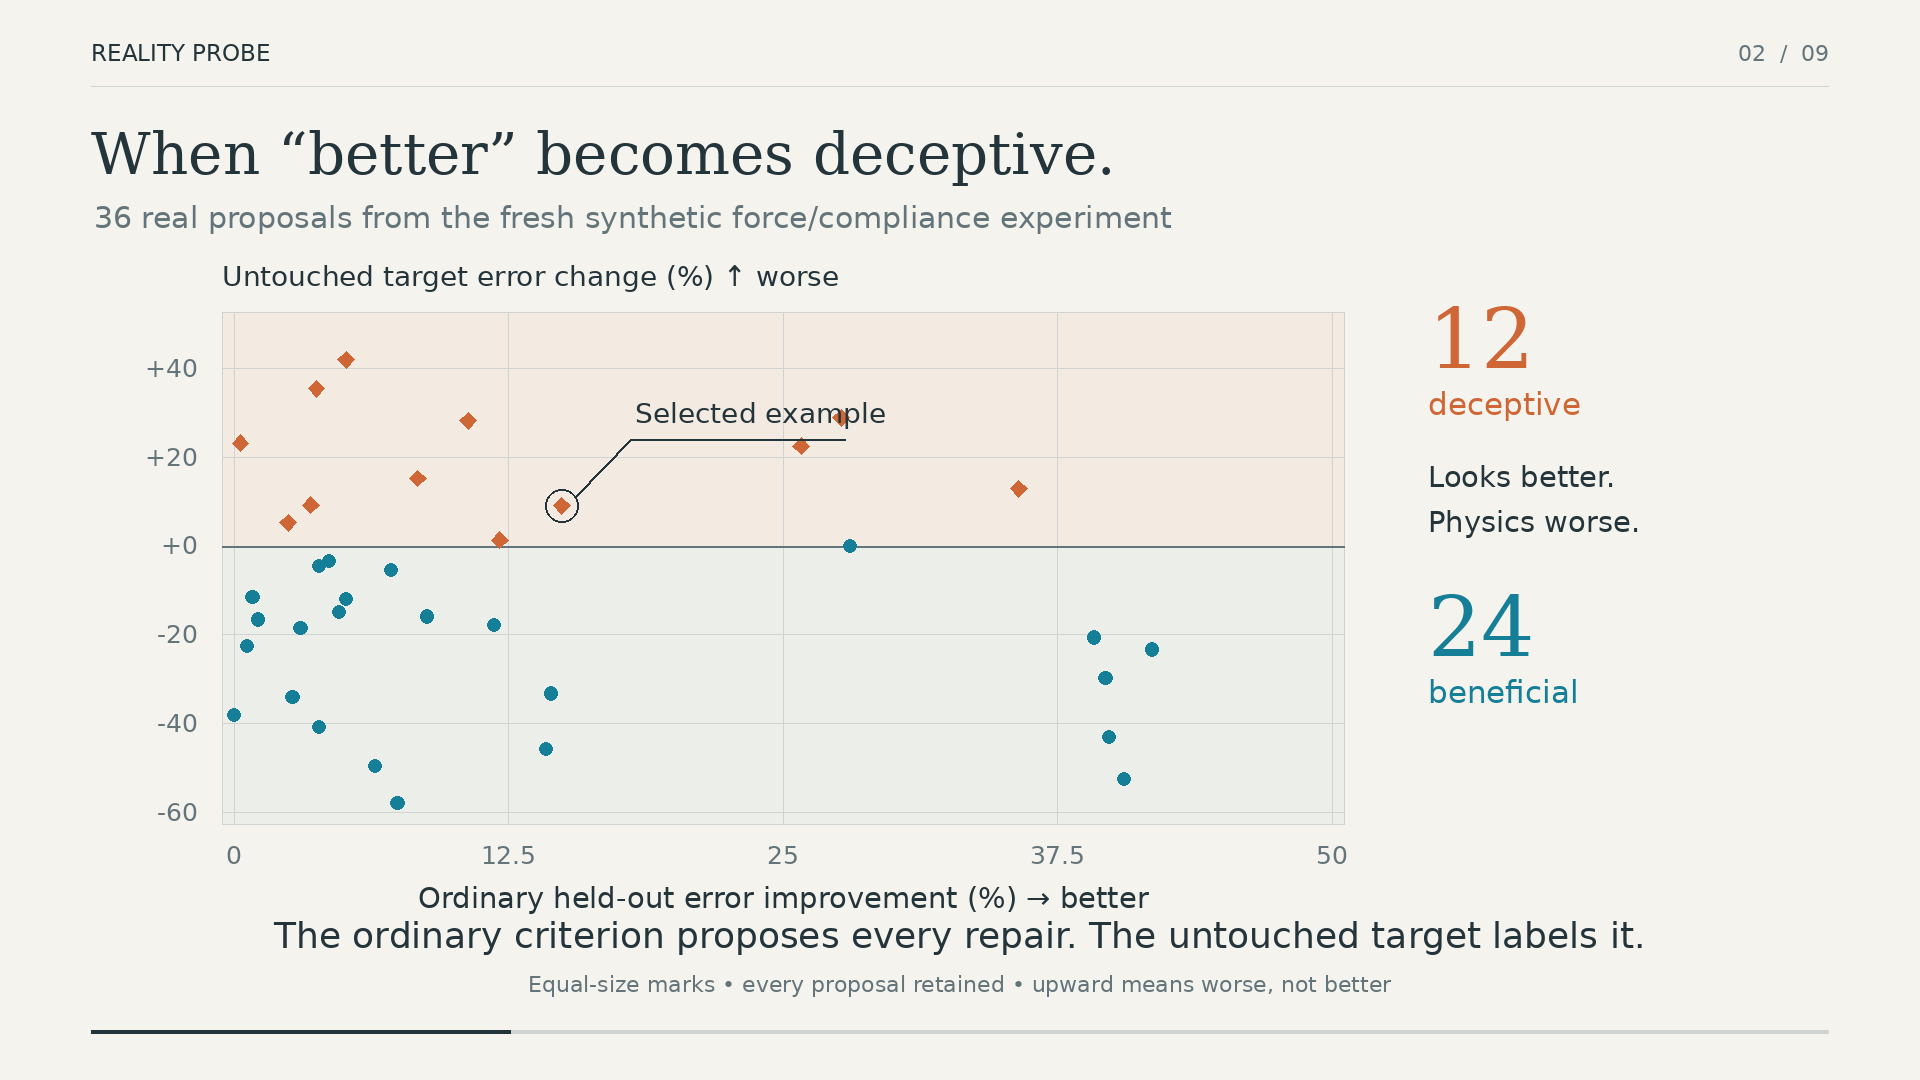
\includegraphics[width=\linewidth]{../docs/readme_assets/03_deception_map.png}
\caption{Fresh force-compliance proposal population. Ordinary held-out improvement and untouched-target behavior disagree for part of the population, producing both deceptive and beneficial rewrites.}
\label{fig:deception-map}
\end{figure}

\subsection{Locked IRIS pendulum protocol and post-final analyses}\label{locked-iris-pendulum-protocol}

The measured positive test uses IRIS \texttt{pendulum\_90}. The tracker, candidate schedule, decision magnitude, and final media are repository-frozen before the 10-video final set is opened. The primary verifier uses the finite-amplitude pendulum period relation. The matched diagnostic baseline uses the small-angle approximation. Each physical video generates 11 controlled SUPPORT/VETO/UNRESOLVED cases, for 110 nested case rows across 10 videos.

Post-final analyses form a separate evidence class. They resample at the physical-video level, compare two additional pendulum residual models, generate GT-hidden proposals from early video segments, vary proposal/probe overlap, propagate recorded rope-length uncertainty, and stress the locked decision under image corruption and temporal downsampling. None of these analyses can replace or retune the locked final result.

\subsection{Frozen IRIS free-fall transfer test}\label{frozen-iris-free-fall-protocol}

The free-fall lane tests a different equation family with a separately frozen protocol. Development uses \texttt{drop\_50/06..10}; validation uses untouched \texttt{drop\_100/06..10}; the designated final set is \texttt{drop\_150/02..10}. The V6.6 policy forbids threshold retuning, tracker changes, candidate changes, or scene substitution after lock. Validation is opened only after the development gate passes. A failed validation permanently removes that split from confirmatory use and prevents the final set from being opened.

\section{Results and Analysis}\label{results-and-analysis}

\subsection{Deceptive repair is a distinct failure
mode}\label{deceptive-repair-is-a-distinct-failure-mode}

D4V and the fresh synthetic OFC population both show why ordinary held-out improvement is not enough. D4V contains 14 deceptive repairs among 36 ordinary-improving proposals; fresh synthetic OFC contains 12 among 36. Those fractions should not be read as a universal deception rate. They serve a more modest purpose: under controlled candidate-generation pipelines, the failure mode exists often enough that a verification rule based only on observation fit cannot ignore it.

\subsection{The stronger DCS hypothesis is not supported in the tested
regime}\label{the-dcs-hypothesis-is-falsified-as-a-general-prospective-verifier}

D1 shows that dark-field rejection can be strong when the experiment is deliberately constructed around that distinction. The strength does not survive the prospective stages. D2 and D3 stay far below the decision magnitude, DCS does not beat the matched ranking baselines, and D4V resolves none of the repair proposals. We treat that as a central result, not an embarrassing corner case. It rules out the stronger story that mechanism-selective cancellation by itself is enough for repair certification in the regime we tested.

The D3 refinement result sharpens this point. Lowering the numerical floor in witness space by several-fold barely changes standardized separation. Whatever is limiting the original witness, it is not simply coarse solver discretization.

\subsection{Orthogonal physical information changes the evidence
scale}\label{orthogonal-physical-information-changes-the-evidence-scale}

\begin{figure}
\centering
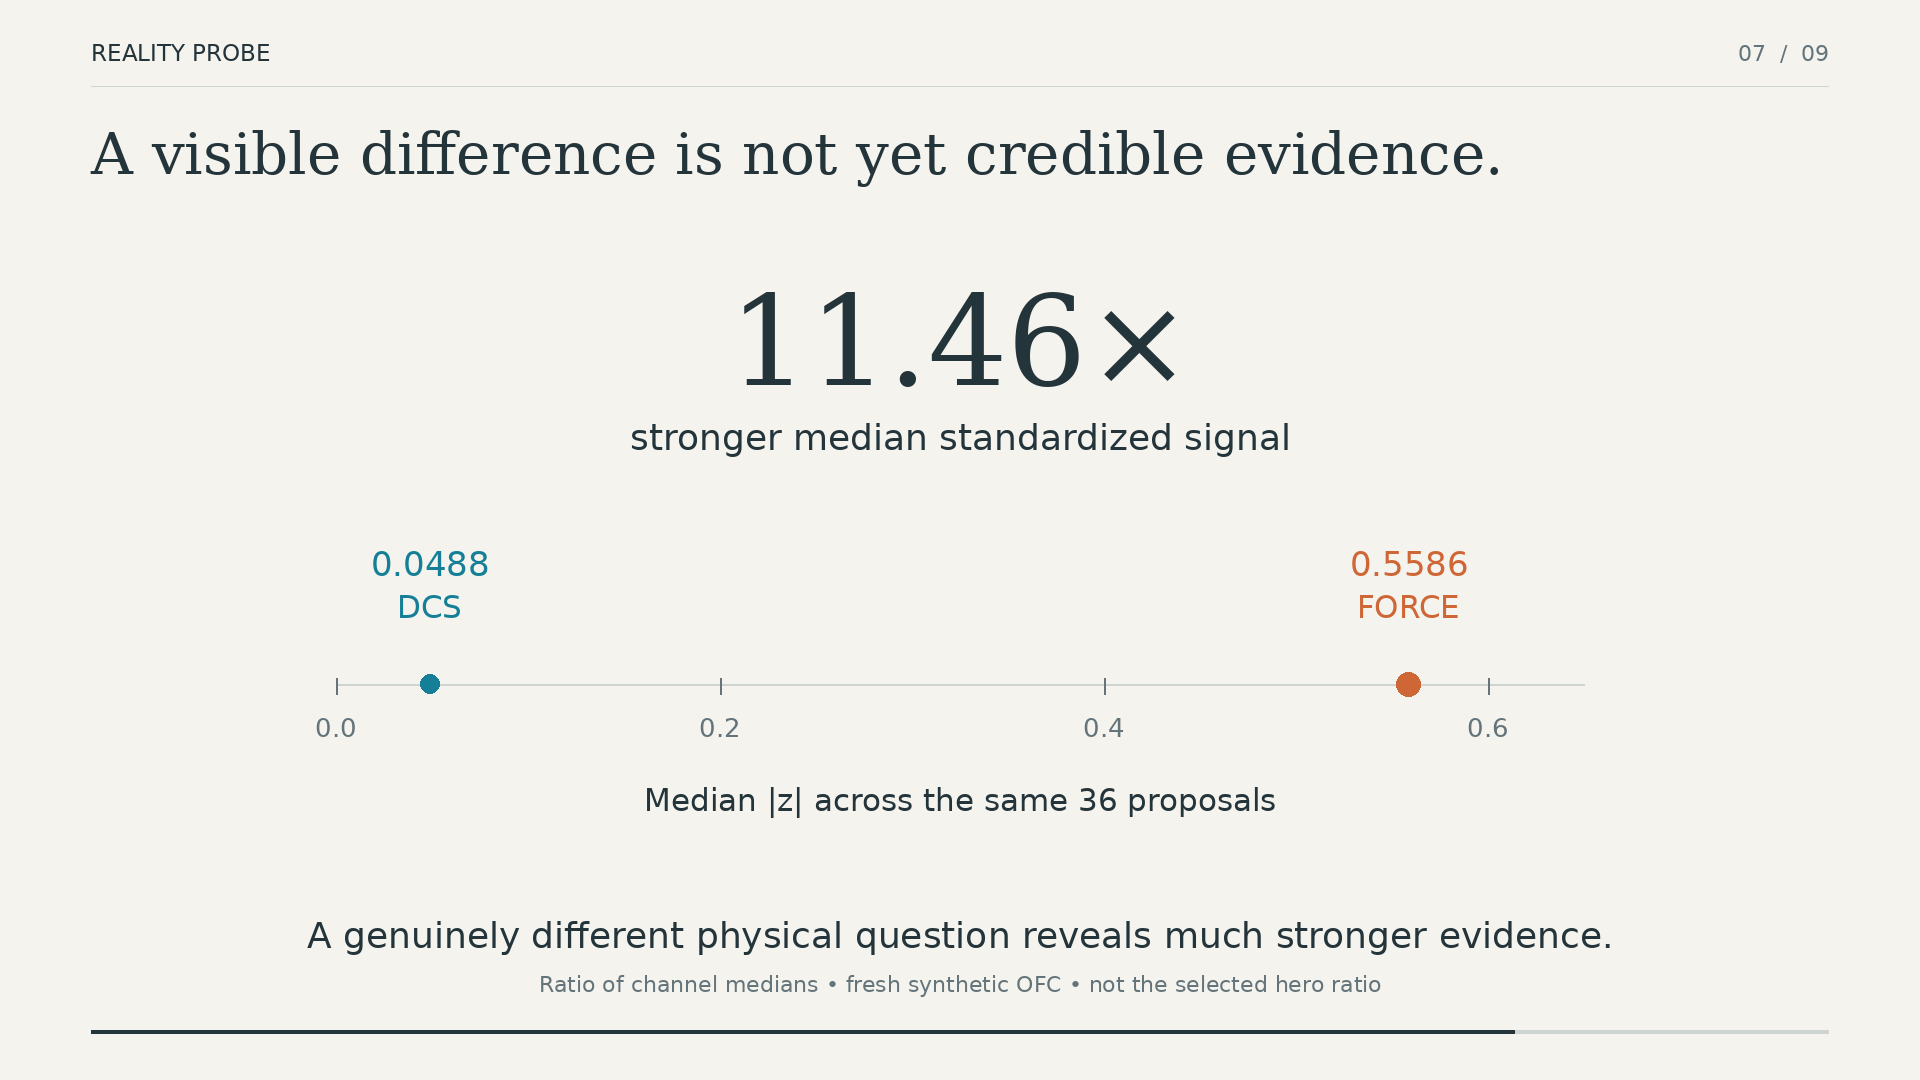
\includegraphics[width=\linewidth]{../docs/readme_assets/10_signal_gain.png}
\caption{Fresh known-force compliance raises the median standardized
signal by 11.46x relative to fresh DCS without changing the frozen
decision rule.}
\end{figure}

The force-compliance experiment shifts the evidence scale in a way the earlier numerical refinements did not. Median standardized magnitude rises to 0.5586, roughly an order of magnitude above the fresh DCS median. Nothing about the decision rule or scoring definition changes; the difference comes from asking a physically different question. We take this as strong evidence that observability is experiment-dependent, while stopping short of claiming that information content is the only factor limiting verification.

\begin{figure}
\centering
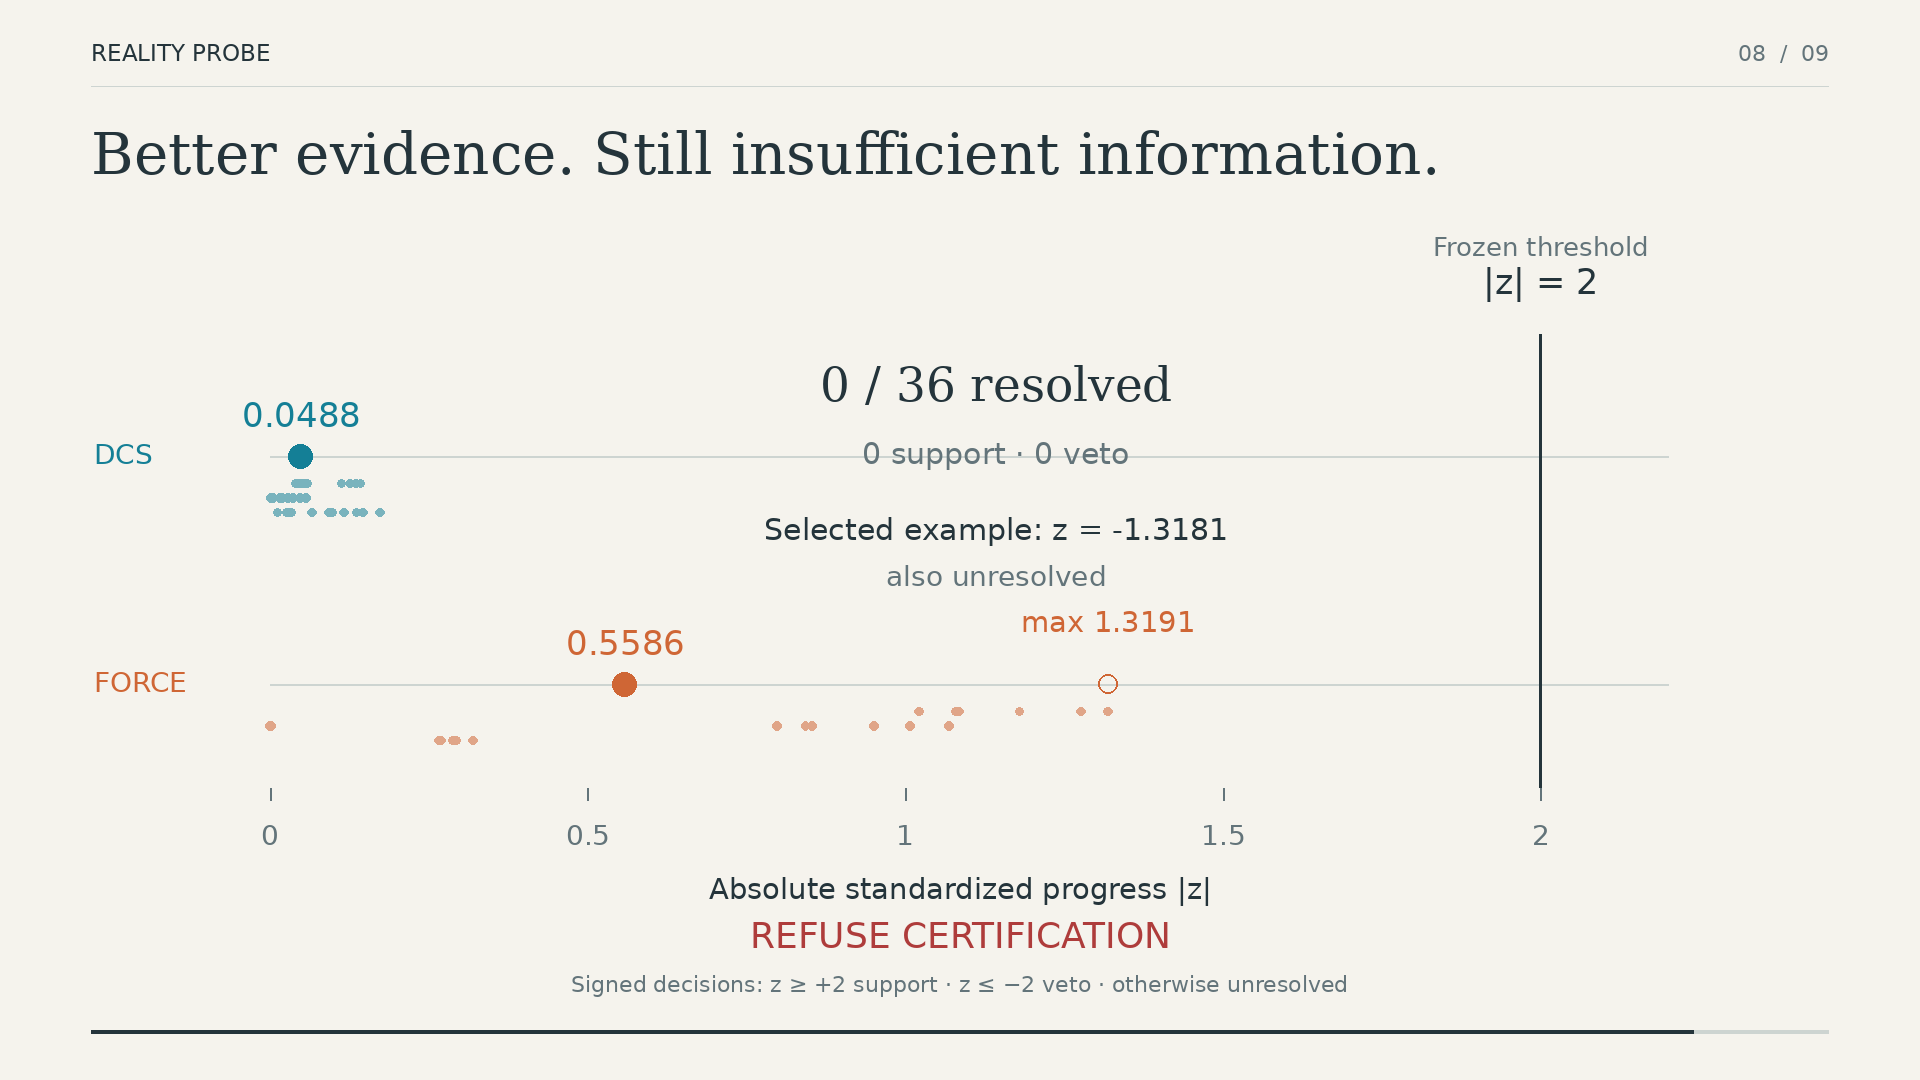
\includegraphics[width=\linewidth]{../docs/readme_assets/11_information_limit.png}
\caption{Information-limit summary from the frozen fresh synthetic orthogonal-information experiment. Known-force compliance increases
standardized evidence substantially, but the strongest case remains
below the frozen decision magnitude.}
\end{figure}

This is why the choice of physical question matters. Kinematic observations may be perfectly adequate for proposing a plausible repair and still be poor at distinguishing that repair from alternatives. A force-controlled test introduces a different constraint on the candidate worlds; in these experiments, that extra constraint is visibly more informative.

\subsection{Stronger evidence is not sufficient
evidence}\label{stronger-evidence-is-not-sufficient-evidence}

The largest magnitude in the fresh synthetic force population is \(|z|=1.31911\), still below the frozen decision boundary. The visualized case has signed force progress \(z=-1.31811\): it moves strongly toward veto but does not reach it. Reality Probe therefore leaves the repair unresolved. We prefer that outcome to lowering the threshold after seeing the partition or pretending that an intermediate score is a definitive physical verdict.

The information-frontier view also prevents a misleading all-or-nothing summary. DCS and force compliance both have 0\% resolved coverage at \(\tau=2\), but they are not equally informative. Their evidence magnitudes, and therefore their remaining distance to the decision boundary, are very different. That difference gives a quantitative direction for future intervention and sensor design even though the present experiment does not justify deployment-level certification.

\section{Discussion}\label{discussion}

\subsection{What is established}\label{what-is-established}

Four conclusions survive the full sequence. First, a rewrite can improve ordinary observations while worsening an untouched physical target. Second, a mechanism-sensitive probe can be implemented correctly and still carry too little information for a reliable decision. Third, changing the interrogation can matter dramatically: known-force compliance raises the synthetic evidence scale, and the locked finite-amplitude pendulum observable produces useful SUPPORT/VETO/UNRESOLVED decisions on fresh real video. Fourth, that success is not automatically transferable. The frozen free-fall replication passes development and then fails untouched validation.

That is narrower than a claim of universal physical correctness, but it is more operationally honest. A persistent captured-world system can keep fitting, verification, and unresolved evidence separate; it can commit or veto when a matched channel supplies enough evidence, and it can abstain or retire a lane when the experiment itself is inadequate.

\subsection{Relation to identifiability and experiment
design}\label{relation-to-identifiability-and-experiment-design}

The force result fits the broader experimental-design principle that model discrimination depends on what is excited and what is measured \citep{asadi2025oed,wang2026identifiability}. We are not introducing that principle. What the experiments expose is its consequence inside a rewrite workflow: verification can fail even when every candidate looks plausible because the experiment does not separate them strongly enough. In that situation the system should not simply pick the highest score. It should collect more informative evidence or remain unresolved.

\subsection{Relation to simulation verification and digital
twins}\label{relation-to-simulation-verification-and-digital-twins}

Simulation-credibility frameworks already distinguish code verification, solution verification, model validation, and uncertainty \citep{oberkampf2007pcmm}. Digital-twin validation similarly asks which counterfactual claims are actually supported by observable validation data \citep{laudy2026digitaltwin}. Reality Probe sits underneath that broader view as an application-specific mechanism. Its scope is a captured world that can be physically edited, where a proposed rewrite is tested through a separately defined verification intervention or observable before commit.

\subsection{Limitations}\label{limitations}

The limitations are not bookkeeping details; several of them define the boundary of the claim.

\begin{itemize}
\item
  \textbf{Fresh prospective force evidence is synthetic.} The orthogonal
  force-compliance experiment uses controlled MPM truth worlds rather
  than a measured force-sensor setup. A real prospective force
  experiment is required for a stronger measured-world claim.
\item
  \textbf{GAUGE is retrospective.} The measured channel contradiction
  motivates the problem and demonstrates that different observables can
  disagree, but it is not an untouched prospective test of DCS or force
  compliance.
\item
  \textbf{The positive measured result is one physical regime.} The
  locked IRIS pendulum result contains 10 fresh videos from one
  \texttt{pendulum\_90} regime. The controlled case rows are nested inside
  those videos and cannot be treated as independent physical experiments.
\item
  \textbf{Pendulum verification is temporally resolution-sensitive.}
  In the full post-final corruption sweep, tested noise, blur, frame
  duplication/drop, occlusion, and crop preserve the clean 81.82\%
  strict accuracy, but temporal downsampling reduces it to 63.64\% at
  30~fps and 45.45\% at 15~fps. Placebo abstention remains 100\%.
  We therefore do not claim robustness to arbitrary acquisition frame
  rates or temporal sampling.
\item
  \textbf{The second real-video domain fails.} The frozen IRIS free-fall
  replication passes low-level tracking quality on all five validation
  videos but misses the physical recovery target badly, with 111.7\%
  median acceleration relative error. We retain that failure, keep the
  validation split retrospective, and leave the final split unopened.
\item
  \textbf{The physical regime is limited.} The principal experiments use
  a fixed deformable MPM setup and selected APIC/PIC candidate families.
  Generalization across constitutive families, contact regimes, and
  solvers is not established.
\item
  \textbf{The decision magnitude is operational.} The value 2 is frozen
  before evaluation and prevents post-hoc threshold tuning, but it is
  not a universal law for all physical verification tasks. A post-hoc
  robustness audit uses the frozen per-proposal ledger: force compliance
  has 14/36 crossings at $\tau=1$ (6 support and 8 veto), while both
  fresh channels have zero crossings for every $\tau\ge1.5$.
\item
  \textbf{DCS synthesis is heuristic.} Lower-moment annihilation is
  exact up to tolerance, but the projected maximin search is not
  globally optimal.
\item
  \textbf{The response-jet interpretation is operational.} The
  implementation estimates order of contact from validated witnesses; it
  does not reconstruct a complete symbolic Taylor tensor.
\item
  \textbf{The selected hero case is post hoc.} It is chosen
  deterministically for explanation and does not influence thresholds,
  aggregate statistics, or the standardized-evidence result.
\item
  \textbf{Spatial residuals are explanatory.} Solver-driven residual
  fields localize response disagreement but are not themselves the DCS
  decision statistic.
\item
  \textbf{Measured DOT parameters are model-conditioned.} The DOT
  benchmark lacks stress-free state, loads, thickness, mass, and
  constitutive ground truth for C2; fitted material values are therefore
  not presented as true cloth properties.
\end{itemize}

\subsection{Future work}\label{future-work}

The next useful experiment is not another tuning pass on the frozen DCS, force-compliance, or failed free-fall partitions. It is a separately frozen measured study whose physical observable is chosen before final data access and is plausibly matched to the rewrite being tested. Independent force sensing, calibrated excitation, modal or frequency-domain response, broader constitutive families, and intervention-specific sensing are natural directions. Whatever comes next should keep proposal generation blind to the confirmatory channel, preserve a SUPPORT/VETO/UNRESOLVED rule declared before the confirming measurements are examined, and leave failed domains failed instead of recycling them into confirmation.

\section{Reproducibility and Implementation
Notes}\label{reproducibility-and-implementation-notes}

The repository records the 2026-09-21 scientific freeze at commit \texttt{a9da8c0aa868}. The one-command runner builds and tests the code, executes the staged experiments, regenerates deterministic figures and tables, validates frozen numerical values, records compiler/system/GPU provenance, and assembles a SHA-256-indexed evidence archive. Paper conclusions are read from machine-readable JSON ledgers rather than reverse-engineered from rounded labels in figures.

The core DCS code is kept separate from the experiment drivers. It includes arbitrary-order lower-moment validation, signed-response application, finite-amplitude counterfactual cumulants, standardized discrepancies, uncertainty propagation, active stencil synthesis, witness-space numerical refinement, and spatial localization. The orthogonal force protocol and fresh synthetic truth worlds are versioned independently of D2/D3/D4V. That separation is there for a practical reason: a negative gate should not disappear because the same data were quietly retuned.

\paragraph{Generative-AI-assisted research workflow.}
OpenAI ChatGPT was used during research for code drafting and debugging,
experiment-orchestration and analysis scripts, visualization/manuscript tooling,
and manuscript revision. AI-generated material was not treated as empirical
evidence. Experimental partitions, thresholds, executed outputs, numerical
claims were checked against committed research artifacts, and cited sources
were checked against publication records before inclusion in the manuscript.

Paper visualizations are generated deterministically. Solver-driven surfaces may use an explicit display magnification so that micrometer-scale motion is visible, but the reported numbers are never scaled. The Stanford Bunny appears only as a visualization carrier where noted and still requires its source attribution; it is not benchmark geometry. The mathematical explainer uses the actual solver body and does not depend on the bunny.

\section{Conclusion}\label{conclusion}

Better observation fit is not the same thing as better physics. Across the controlled repair populations, some ordinary-improving rewrites make an untouched physical target worse. Reality Probe turns that mismatch into an explicit evidence transaction, with DCS as one tested mechanism-selective probe rather than the framework itself. The negative D2/D3/D4V sequence shows that a valid probe can still be information-poor; the force-compliance experiment shows that changing the physical channel can raise the evidence scale by 11.46$\times$ without yet crossing the frozen decision boundary. The locked IRIS pendulum result provides the positive measured case: 90/110 correct controlled decisions versus 40/110 for the matched small-angle baseline across 10 fresh videos, with all 10 placebo cases correctly left unresolved. The subsequent free-fall replication then fails untouched validation and stays failed. Taken together, the evidence supports a conditional systems claim rather than a universal verifier: when a physical channel is well matched to the requested rewrite, Reality Probe can support or veto; when it is not, the right behavior is to remain unresolved or retire that verification lane.

\section*{Acknowledgments}

\textbf{Generative AI disclosure.}
OpenAI ChatGPT was used as a research and writing assistant during the
development of this work, including drafting and revising manuscript
text, generating and debugging code, assisting with experiment
orchestration and analysis scripts, preparing tables, figures, and
visualization/manuscript tooling, and manuscript formatting. The author
reviewed the generated material, validated the reported experiments and
numerical evidence against the frozen research artifacts, checked the
references used in the manuscript, and takes responsibility for the
final content of the work.

\bibliographystyle{ACM-Reference-Format}
\bibliography{references}

\end{document}
